\documentclass{book}

\usepackage[utf8]{inputenc} %caràcters en català
\usepackage[printonlyused]{acronym} %acrònimcs
\usepackage{hyperref} %hiperlinks
\usepackage{glossaries} %glossaris
\usepackage{enumitem} %per enumerar i fer llistes
\usepackage{graphicx} %incloure figures
\usepackage{geometry} %marges de la pagina
\usepackage{pdfpages} %incloure pdfs dins el document
\usepackage{eurosym} \DeclareUnicodeCharacter{20AC}{\euro} %pel simbol €
\usepackage{setspace} %Per l'interlineat
\usepackage{subcaption} %Per posar imatges una al costat de l'altre
\usepackage{fancyhdr} %Capçalera i Peu de pagina maco

\newcommand*\barrier{
\includegraphics[scale=0.5]{red_lightning.png}} %simbol llamp
\newcommand*\blacktriangle{
\includegraphics[scale=0.05]{blacktriangle.png}}

%Mides document
\geometry{
 a4paper,
 total={210mm,297mm},
 left=30mm, %interior
 right=20mm, %exterior 
 top=25mm,
 bottom=25mm,
 includehead, includefoot %Incloure capçalera i peu dins dels marges 
}

%Format de les pàgines d'inici de capítol
\fancypagestyle{plain}{
	\fancyhf{} % clear all header and footer fields
	\fancyhead[LE, RO]{\thepage} %Part exterior
	\fancyhead[LO, RE]{Estudi de l'UX sobre les aplicacions de gestió de despeses personal per Android} %Part interior
	\renewcommand{\footrulewidth}{0pt}
}

%Format de la capçalera i del peu pàgina
\pagestyle{fancy}
\fancyhead[LE, RO]{\thepage} %Part exterior
\fancyhead[LO, RE]{Estudi de l'UX sobre les aplicacions de gestió de despeses personal per Android} %Part interior
%\fancyfoot[LE, RO]{\leftmark} %Part exterior
%\fancyfoot[LO, RE]{Arnau Villoro Bort} %Pert interior
\fancyfoot[C]{} %Eliminar part central
\fancyfoot[LE, RO]{
\includegraphics[height=1.5cm]{logo_etseib.png}} %Logo
\textheight = 225mm %Deixar espai pel logo reduint espai pel text
\footskip = 22mm %Deixar espai pel logo augmentant el peu de pagina


%Noms de les parts
\renewcommand{\chaptername}{Capítol}
\renewcommand{\contentsname}{Sumari}
\renewcommand{\listtablename}{Llista de taules}
\renewcommand{\figurename}{Figura}
\renewcommand{\tablename}{Taula} 

%Colors a les taules
\usepackage{xcolor, colortbl}
\definecolor{blue_table_1}{RGB}{220,230,241}
\definecolor{blue_table_2}{RGB}{141,180,226}
\definecolor{blue_table_3}{RGB}{83,141,213}

%Mides i format dels paràgrafs i del text
\setlength{\parindent}{1em} %Paragraph Indentation: espai horitzontal previ a l'inici d'un paragraf
\setlength{\parskip}{1em} %Paragraph spacing: espai entre paragraphs
\onehalfspace %Line spacing: interlineat

%Exemples macos: http://tex.stackexchange.com/questions/1319/showcase-of-beautiful-typography-done-in-tex-friends

\title{Estudi de l'experiència d'usuari sobre les aplicacions de gestió de despeses personals per Android}
\author{Arnau Villoro Bort}

\makeglossaries

%------------------------------------------------------------------
\begin{document}

\newcommand{\blueA}{\cellcolor{blue_table_1}}
\newcommand{\blueB}{\cellcolor{blue_table_2}}
\newcommand{\blueC}{\cellcolor{blue_table_3}}
\newcommand{\headA}[1]{\multicolumn{1}{|c|}{\blueA \textbf{#1}}}
\newcommand{\headB}[1]{\multicolumn{1}{|c|}{\blueB \textbf{#1}}}
\newcommand{\headC}[1]{\multicolumn{1}{|c|}{\blueC \textbf{#1}}}
\newcommand{\noBorde}[1]{\multicolumn{1}{#1}{}}


\frontmatter


\includepdf{Portada.pdf}

%\maketitle

\chapter*{Resum} \label{sec:Resum}
\addcontentsline{toc}{chapter}{Resum}

En aquest projecte s'ha fet un estudi d'Experiència d'Usuari (UX) sobre les aplicacions de gestió de despeses personals per a \gls{Android}. Per a tal fi, en primer lloc s'ha definit què és i com es fan els estudis d'UX, explicant amb detall en que consisteixen les seves 4 etapes, que són: Anàlisi, Disseny, Implementació i Avaluació.

L'estudi en si ha començat analitzant com els usuaris gestionen les seves despeses i la seva satisfacció amb les aplicacions existents més rellevants per a \gls{Android}. Utilitzant aquest anàlisi s'ha definit els requeriments necessaris per a una aplicació per a la gestió de les despeses personals. Després d'aquest anàlisi previ s'ha fet un procés iteratiu on es dissenyaven i s'implementaven prototips d'aquesta aplicació, augmentant-ne la fidelitat i el detall d'aquests a cada iteració. A continuació s'utilitzaven aquests prototips amb usuaris per a validar que satisfeien les seves necessitats, modificant els requeriments inicials si era necessari. 

Com a resultat d'aquest procés iteratiu s'ha creat un prototip programat que implementa les funcions més importants d'una aplicació per a gestionar les despeses domèstiques. Llavors s'ha comparat l'experiència d'usuari que proporcionava aquest prototip respecte les aplicacions ja existents al mercat. El resultat és un prototip que proporciona la millor UX d'entre les aplicacions ja existents.

Per a poder dissenyar aquest prototip ha calgut modelitzar el problema de la resolució dels deutes en grup, alhora que dissenyar i implementar un algoritme que ho solucioni. També s'ha comprovat el seu cost d'execució amb diversos jocs de dades. 

Finalment s'han descrit els passos que caldria seguir per a poder passar del prototip programat a una aplicació completament funcional que es pugui penjar a les botigues d'aplicacions. 




\tableofcontents

\chapter*{Llista d'acrònims}
\label{sec:glossary}
\addcontentsline{toc}{chapter}{Glossari}

%INFO: http://en.wikibooks.org/wiki/LaTeX/Glossary

\begin{acronym}
\acro{PFC}{Projecte Final de Carrera}
\acro{UX}{\textit{User Experience}}
\acro{UI}{\textit{User Interface}}
\acro{CSV}{\textit{Comma-Separated Values}}
\acro{WAAD}{\textit{Work Activity Affinity Diagram}}
\end{acronym}


\newglossaryentry{Android}
{
name = Android, description = {Sistema operatiu mòbil amb el qual funcionen la majoria de telèfons mòbils \cite{Android_OS}}
}

\newglossaryentry{barrier}
{
name = barrera, description = {És un problema que interfereix amb les operacions que l'usuari executa normalment}
}

\newglossaryentry{affinity_diagram}
{
name = diagrama d'afinitat, description = {És una representació gràfica i jeràrquica que serveix per mostrar un resum extret de una gran quantitat d'informació quantitativa i qualitativa.}
}

\newglossaryentry{WAAD}
{
name = \textit{Work Activity Affinity Diagram}, description = {És un diagrama d'afinitat que serveix per filtrar i organitzar les notes d'activitat de treball extretes a l'anàlisi contextual. Serveix per mostrar les notes agrupades i organitzades segons similituds entre elles.}
}

\newglossaryentry{conceptual_design}
{
name = disseny conceptual, plural = dissenys conceptuals, description = {És un tema, noció o idea amb el propòsit de comunicar una visió del disseny del sistema o producte. És la part del disseny del sistema que porta el model mental del dissenyador a la vida.}
}

\newglossaryentry{User_Experience}
{
name = \textit{user experience} o experiència d'usuari, description = {És la totalitat de l'efecte o efectes que sent (o experimenta) internament l'usuari com a resultat de la interacció, i del context d'ús, amb el sistema, dispositiu o producte.}
}

\newglossaryentry{Google_play}
{
name = Google Play, description = {Botiga virtual de Google en la qual es troben les aplicacions per a dispositius mòbils que funcionen amb \gls{Android} (\url{https://play.google.com/store/apps})}
}

\newglossaryentry{Holo}
{
name = Holo, description = {Són unes directrius de disseny per a les aplicacions d'\gls{Android} que es van crear amb la versió 4.0.}
}

\newglossaryentry{contextual_inquiry}
{
name = \textit{investigació contextual}, description = {És una activitat que forma part d'un estudi d'UX que consisteix en recopilar informació detallada sobre com els usuaris interaccionen amb un producte/sistema. La seva finalitat és poder construir i/o millorar el producte/sistema i és du a terme mitjançant entrevistes i observacions dels usuaris.}
}

\newglossaryentry{inventari_tasques}
{
name = inventari de tasques jeràrquic, description = {És un model d'ús que representa les diferents tasques que es poden executar de forma jeràrquica. Dins l'estructura un fill és una subtasca del seu pare, no una tasca posterior en el temps.}
}

\newglossaryentry{Material}
{
name = Material Design, description = {Són unes directrius de disseny per a les aplicacions d'Android que es van crear amb la versió 5.0 per a substituir i millorar Holo. Per més informació \url{http://developer.android.com/design/material/index.html}}
}

\newglossaryentry{flow_model}
{
name = model de flux, description = {És una representació gràfica que explica com les diferents entitats es comuniquen per tal d'aconseguir que el treball es realitzi.}
}

\newglossaryentry{models_interaccio_tasques}
{
name = models d'interacció de les tasques, description = {És un model d'ús que representa l'execució pas a pas d'una tasca, incloent l'objectiu de la tasca, catalitzadors i les accions dels usuaris.}
}

\newglossaryentry{mockup}
{
name = \textit{mockup}, description = {És una representació estàtica de fidelitat mitja o alta.  Representa l'estructura de la informació i demostra les funcionalitats bàsiques d'una manera estàtica.}
}

\newglossaryentry{workActivityNotes}
{
name = nota d'activitats de treball, plural = notes d'activitats de treball, description = {Es tracta de notes que parafrasegen i representen la opinió d'un usuari per a facilitar la comprensió de la opinió dels usuaris.}  
}

\newglossaryentry{work_role}
{
name = rol de treball, plural = rols de treball, description = {Corresponen als deures, funcions i activitats que desenvolupa una persona amb cert lloc de treball.}  
}

\newglossaryentry{persona}
{
name = personatge, description = {És una representació utilitzada en el disseny per a representar una persona fictícia amb un rol de treball concret. Serveix per a ajudar als dissenyadors a imaginar-se millor per a qui estan dissenyant}  
}

\newglossaryentry{prototip}
{
name = prototip, description = {És una representació navegable del producte final i normalment és de fidelitat mitja o alta. Simula la interacció amb la interfície d'usuari i permet que l'usuari experimenti interactuant amb la interfície i el contingut. També permet que provi les principals interaccions d'una manera molt similar al producte final.}
}

\newglossaryentry{prototip_h}
{
name = prototip horitzontal, plural = prototips horitzontals, description = {És un prototip què té moltes funcions però amb una profunditat baixa en quan a funcionalitat.}
}

\newglossaryentry{prototip_l}
{
name = prototip local, plural = prototips locals, description = {És un prototip que només implementa unes poques funcions i amb poca profunditat en quan a funcionalitat.}
}

\newglossaryentry{prototip_v}
{
name = prototip vertical, plural = prototips verticals, description = {És un prototip amb una profunditat alta de funcionalitat però que es centra només en poques funcions}
}

\newglossaryentry{sketch}
{
name = \textit{sketch}, description = {És un dibuix ràpid que es realitza a mà alçada que reprodueix un concepte, idea o la generalitat d'un projecte de manera molt senzilla. És una representació de baixa fidelitat} 
}

\newglossaryentry{work}
{
name = treballar, description = {Dins de l'àmbit d'UX, és interactuar o utilitzar el sistema/producte.} 
}

\newglossaryentry{wireframe}
{
name = \textit{wireframe}, description = {És una representació estàtica de baixa fidelitat d'un disseny. Mostra la estructura general així com les diferents parts que la componen representat per caixes o formes}
}




\printglossary


\chapter*{Apps}
\label{sec:apps}

\begin{tabular}{ | l | c | l | l | }
\hline
\textbf{Núm.} &  & \textbf{Nom} & \textbf{Autor} \\
\hline
App 1 & 
\includegraphics[scale=0.05]{A01_icon.png} & \href{https://play.google.com/store/apps/details?id=com.expensemanager}{Expense Manager} & Bishinews \\

App 2 & 
\includegraphics[scale=0.05]{A02_icon.png} & \href{https://play.google.com/store/apps/details?id=at.markushi.expensemanager}{Expense Manager} & Markus Hintersteiner \\

App 3 & 
\includegraphics[scale=0.05]{A03_icon.png} & \href{https://play.google.com/store/apps/details?id=com.bruno.myapps.droidwallet}{Droid Wallet} & William Bruno \\

App 4 & 
\includegraphics[scale=0.05]{A04_icon.png} & \href{https://play.google.com/store/apps/details?id=com.code44.finance}{Financius - Expense Manager} & Mantas Varnagiris \\

App 5 & 
\includegraphics[scale=0.05]{A05_icon.png} & \href{https://play.google.com/store/apps/details?id=com.handyapps.expenseiq}{Expense IQ} & Handy Apps \\

App 6 & 
\includegraphics[scale=0.05]{A06_icon.png} & \href{https://play.google.com/store/apps/details?id=com.techahead.ExpenseManager}{Diario Gasto Gerente (Daily Expense Manager)} & Gullak \\

App 7 & 
\includegraphics[scale=0.05]{A07_icon.png} & \href{https://play.google.com/store/apps/details?id=com.bookmark.money}{Money lover - Expense Manager} & ZooStudio   \\

App 8 & 
\includegraphics[scale=0.05]{A08_icon.png} & \href{https://play.google.com/store/apps/details?id=com.kpmoney.android}{AndroMoney (Expense Track)} & AndroMoney \\

App 9 & 
\includegraphics[scale=0.05]{A10_icon.png} & \href{https://play.google.com/store/apps/details?id=cz.destil.settleup}{Settle up} & David Vávra \\

App 10 & 
\includegraphics[scale=0.05]{A11_icon.png} & \href{https://play.google.com/store/apps/details?id=com.Splitwise.SplitwiseMobile}{Splitwise} & Splitwise \\

App 11 & 
\includegraphics[scale=0.2]{A12_icon.png} & Expensor & Arnau Villoro \\
\hline
\end{tabular}
\chapter{Prefaci} \label{Prefaci}

Des que tinc memòria he estat molt interessat en la gestió de la informació i de les dades, així com l'enregistrament d'aquestes. No és estrany doncs, el meu interès per a gestionar i controlar les meves despeses. Amb l'aparició dels \glspl{smartphone}, o telèfons intel·ligents, portar un registre de despeses va passar a ser quelcom bastant fàcil. Només calia descarregar-se una aplicació per al mòbil i amb aquesta podies fàcilment apuntar totes les despeses. 

Més endavant vaig descobrir que també hi havia aplicacions que permetien dividir fàcilment les despeses fetes en grup, per a gestionar, per exemple, un viatge amb els amics. Però amb el temps em vaig adonar que, tot i provar-ne moltes, no hi havia cap aplicació que satisfés les meves necessitats. Va ser per això que, cap al Octubre del 2013, vaig decidir que havia de crear jo la meva aplicació.

El problema va ser que en aquell moment em faltaven molts coneixements, però el que em mancava, ho compensava amb moltes ganes i il·lusió. Mig any després i amb moltes hores invertides, ja havia aprés a usar el llenguatge Java, així com a fer aplicacions per a \gls{Android}. 

Paral·lelament vaig començar a buscar idees sobre que podia fer el meu \ac{PFC}. Fins que un bon dia vaig veure unes propostes del Sergi (el meu tutor del \ac{PFC}) a la borsa de projectes, sobre coses relacionades amb \gls{Android} i aplicacions, i que estava obert a propostes. 

A partir d'aquí només va caldre una reunió per a entendre'ns, i així va ser com vam començar aquest projecte. 






\mainmatter
\chapter{Introducció}

\section{Objectius del projecte}
L'objectiu d'aquest \ac{PFC} és fer un estudi de l'Experiència d'Usuari o \textit{User Experience}(UX) per una aplicació que serveixi per a gestionar les despeses personals domèstiques. Prèviament a l'estudi, es busca definir com es fan actualment els estudis \ac{UX} i quines parts tenen aquests tipus d'estudis. Després es procedirà amb l'estudi en si, on es busca definir com ha de ser una aplicació d'aquest tipus per a que garanteixi una bona \ac{UX}.

Concretament es busca dissenyar una aplicació que:
\begin{itemize}
\item Permeti enregistrar despeses i ingressos tot categoritzant-los.
\item Serveixi per a recordar els deutes (positius o negatius) que es tenen amb diverses persones.
\item Faciliti la gestió de despeses grupals alhora que permeti saldar els deutes minimitzant les transaccions entre els membres.
\item Sigui intuïtiva i senzilla de fer servir.
\item Visualment sigui agradable i minimalista per a que sigui agradable i còmode per a l'usuari.
\item Agradi als usuaris en general.
\end{itemize}

Per a dissenyar l'aplicació primer s'analitzarà com interaccionen els usuaris amb les aplicacions de gestió de despeses, per extreure'n les necessitats i les funcionalitats necessàries. Finalment es comprovarà la idoneïtat del disseny creat.

Finalment també es busca resoldre els problemes d'enginyeria que es puguin derivar de les diverses funcions que haurà d'implementar l'aplicació. 

\section{Abast del projecte}
En aquest projecte s'estudiarà l'\ac{UX} per al tipus d'aplicacions esmentat tot definint quines utilitats i funcionalitats ha de tenir l'aplicació i com ha de ser la \ac{UI}. L'estudi s'enfocarà únicament en una aplicació per a \glspl{smartphone} que funcionen amb \gls{Android}, l'actual sistema operatiu més utilitzat\cite{Android_OS} en \glspl{smartphone} o telèfons intel·ligents. 
Finalment en quan al desenvolupament de l'aplicació, no es considera factible crear-la sencera amb totes els requeriments que es puguin deduir amb l'estudi de l'\ac{UX}. És per això que es faran proves de concepte, creant un o varis prototips que s'apropin el màxim possible a com hauria de ser l'aplicació. 

\chapter{Experiència d'Usuari}
\section{Que s'entén per Experiència d'Usuari}
Segons Rex Hartson (2012, p. 19)\cite{UX_Book}, l'\ac{UX} és la totalitat de l'efecte o efectes que sent (o experimenta) internament l'usuari com a resultat de la interacció, i del context d'ús, amb el sistema, dispositiu o producte. És a dir, una bona \ac{UX} es produirà quan l'usuari gaudeixi interaccionant i utilitzant el dispositiu o producte. Interacció i ús s'empren en un sentit molt ampli, ja que inclouen veure, tocar, pensar sobre el producte/dispositiu o fins i tot admirar-lo. 
A més, l'\ac{UX} també engloba la usabilitat i la utilitat. Certament l'usuari sent internament parts de la usabilitat, com l'augment de productivitat, però hi ha certes manifestacions de usabilitat, com podria ser el temps invertit en la tasca, que representa un component no necessàriament experimentat internament per l'usuari.

\section{Com s'estudia l'Experiència d'Usuari?}
L'\ac{UX} no pot ser dissenyada ja que depèn, no només del producte en si mateix, sinó que també depèn de l'usuari i la situació en la que l'utilitza [Smashing Magazine, 2012, p. 25-28]\cite{Smashing_User_Experience_Design}. I és que no és possible dissenyar ni l'usuari ni la situació. Però el que si es pot fer és dissenyar per a una bona \ac{UX} i és això el que s'entén per fer un estudi d'\ac{UX}. Per a fer-ho es segurian les 4 activitats elementals o etapes que Rex Harton proposa en el seu llibre d'\ac{UX} \cite{UX_Book}, que són anàlisi, disseny, implementació i avaluació, tal i com es pot veure a la figura \ref{fig:UX_lifecycle}. Per tal d'aconseguir proporcionar una bona \ac{UX} aquestes activitats és duen a terme de forma iterativa, ja que no sempre és possible trobar un bon disseny al primer intent.

\begin{figure}[htp]
\centering
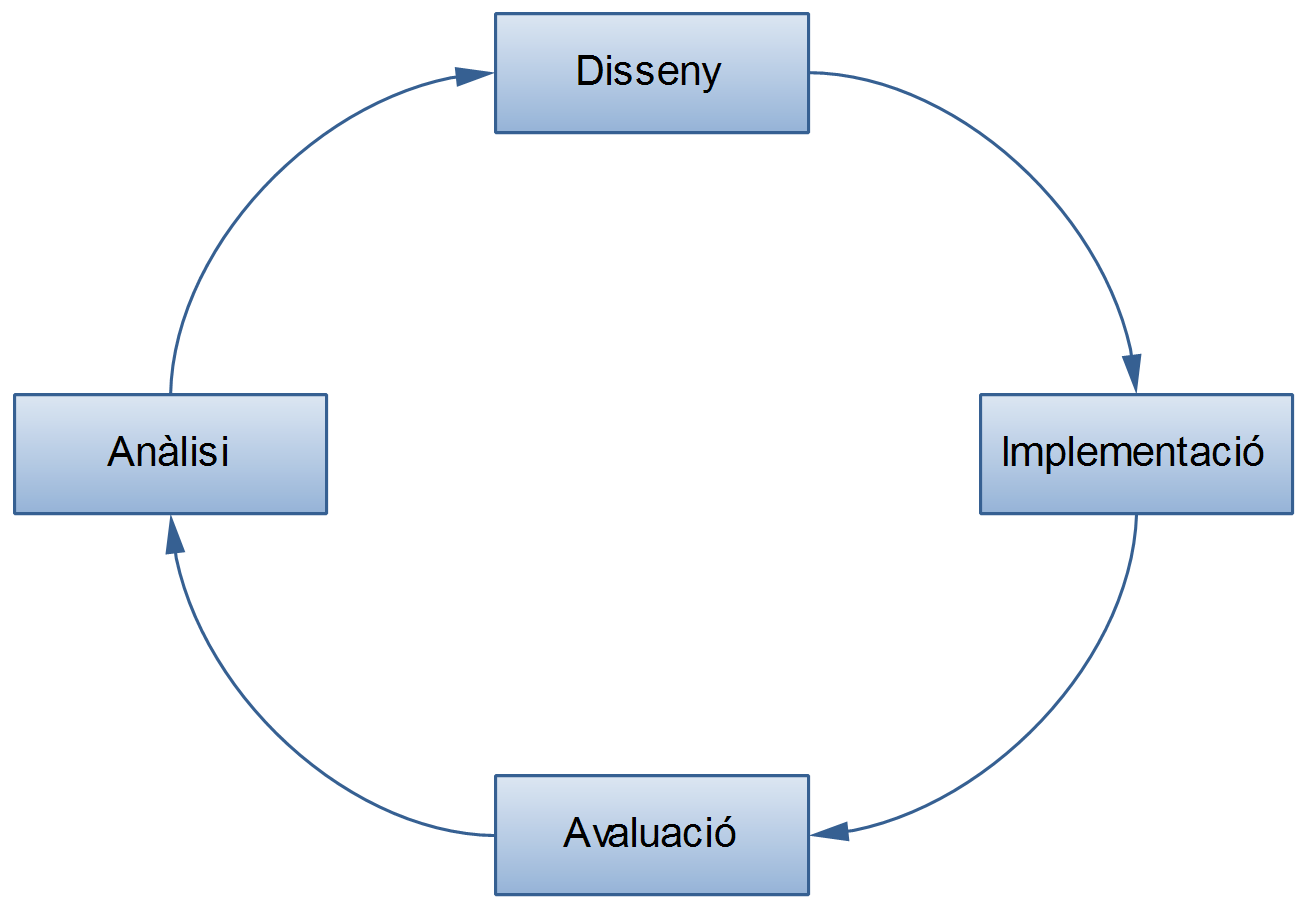
\includegraphics[scale=0.6]{UX_wheel.png}
\caption{Activitats a seguir per a dissenyar garantint una bona \ac{UX}}\label{fig:UX_lifecycle}
\end{figure}

Aquestes quatre activitats, a grans trets, consisteixen en:
\begin{description}
\item [Anàlisi] Es basa en entendre les necessitats de l'usuari que utilitzarà el producte.
\item [Disseny] Consisteix en la creació de dissenys conceptuals determinant la interacció, el comportament i l'aparença del producte.
\item [Implementació] Correspon a la creació de prototips.
\item [Avaluació] Es tracta de comprovar si el disseny satisfà les necessitats dels usuaris que s'han determinat.
\end{description}

\subsection{Anàlisi}\label{sec:analisi}
L'objectiu general d'aquesta activitat és definir com són les usuaris potencials. Un cop definits, serviran per a poder extreure com interaccionaran amb el producte, quines necessitats tindran i en conseqüència els requeriments del producte, tal com afirma Rich Fulcher \cite{user_centred_design}.

Dins de l'anàlisi hi ha quatre subactivitats o passos a seguir:

\subsubsection{Investigació contextual}\label{subsec:investigacio_contextual}
Durant la investigació contextual s'estudia com les persones treballen o interactuen amb el producte en el seu entorn de treball. Per treball s'entén l'ús del producte en si i per entorn de treball, l'entorn en que habitualment s'usa aquest. S'utilitzen aquests termes independentment de la tipologia del producte. És a dir, encara que el producte fos un joc, al fet d'utilitzar-lo se l'anomena treballar. 

Durant la investigació contextual es tracta d'investigar i descobrir com l'usuari treballa en l'entorn habitual i això no es pot determinar enquestant als usuaris. El problema és que la descripció que pugi fer un usuari de com treballa no és fiable. La forma correcta d'investigar és observant com els usuaris treballen i entrevistant-los mentre ells duen a terme aquesta activitat. Per tant es tracta de:

\begin{itemize}
\item Preparar i realitzar visites de camp a l'entorn de treball, on el producte serà utilitzat, de l'usuari/client.
\item Observar i entrevistar els usuaris mentre treballen.
\item Indagar en l'estructura de la pròpia pràctica de treball de l'usuari.
\item Aprendre com la gent treballa en l'entorn en el qual treballarà amb el producte a dissenyar.
\item Extreure notes detallades de les observacions i entrevistes.
\end{itemize}

Durant la investigació contextual és important no preguntar als usuaris que volen o necessiten. En aquesta etapa no es busca que necessiten sinó observar i entrevistar els usuaris en el seu entorn de treball sobre com treballen.


\subsubsection{Anàlisi contextual}\label{subsec:analisi_contextual}
L'essència d'aquest pas és el processament, la interpretació i l'anàlisi de la informació aconseguida a la investigació contextual (apartat \ref{subsec:investigacio_contextual}). Això s'aconsegueix a base de:

\begin{itemize}
\item Crear un model de flux.
\item Sintetitzar la informació en \glspl{workActivityNotes}.
\item Construir un \ac{WAAD} a partir de les \glspl{workActivityNotes}.
\end{itemize}

El model de flux és una representació gràfica que explica com les diferents entitats es comuniquen per tal d'aconseguir que el treball es realitzi. Per a poder crear el model de flux cal identificar els rols de treball. Un rol de treball correspon als deures, funcions i activitats que desenvolupa una persona amb cert lloc de treball.

\begin{figure}[htp]
\centering
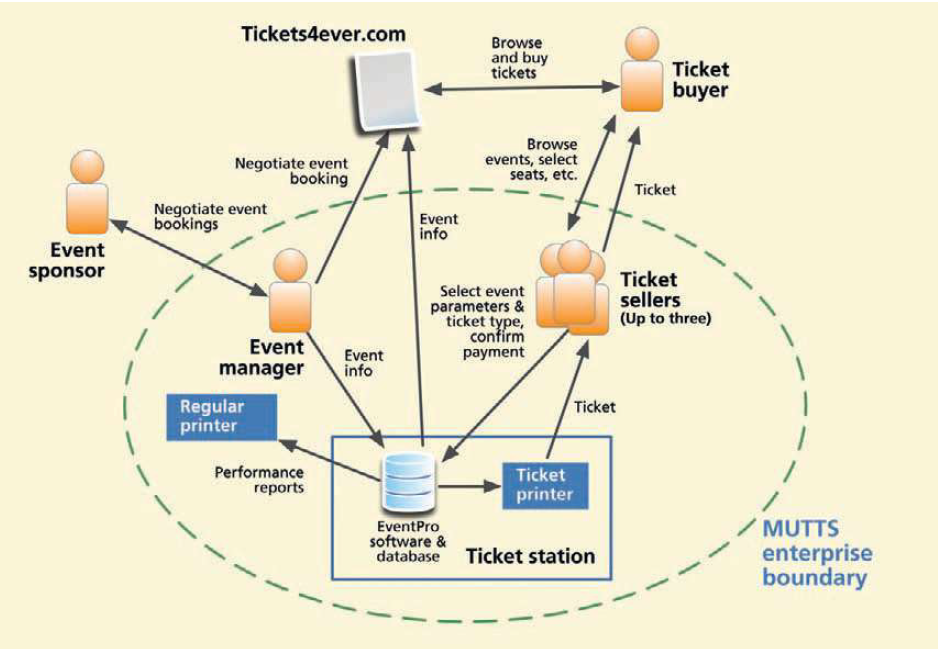
\includegraphics[scale=0.6]{flow_model_example.png}
\caption{Exemple de model de flux.}\label{fig:flow_model_example}
\end{figure}

Paral·lelament a la creació del model de flux, cal sintetitzar la informació en brut que s'ha extret a la investigació contextual. Això es fa creant \glspl{workActivityNotes} les quals, un cop tota la informació ha estat processada, han de representar tota la informació abans extreta. Aquestes notes es caracteritzen per estar escrites en primera persona (des de la perspectiva de l'usuari) parafrasejant i sintetitzant la opinió d'aquest. Cada nota ha de ser concisa i compacta, de manera que expressi una sola idea. Un exemple d'aquestes notes és el de la figura \ref{fig:workActivityNote1}. Com es pot veure cal etiquetar les notes amb un identificador representant l'usuari del qual provenen.

\begin{figure}[htp]
\centering
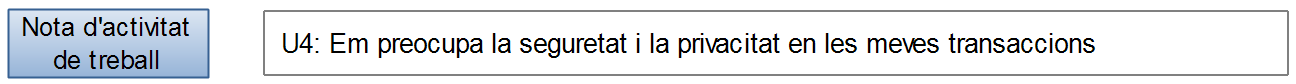
\includegraphics[scale=0.3]{WorkActivityNotes1.png}
\caption{Exemple d'una nota d'activitats de treball}\label{fig:workActivityNote1}
\end{figure}

Les \glspl{workActivityNotes} serveixen per a construir el \ac{WAAD}. Aquest diagrama consisteix en l'agrupació de les notes segons grups o afinitats segons la perspectiva de l'usuari. L'objectiu d'aquest diagrama és transmetre de forma clara i ràpida la opinió dels usuaris. El que es busca es que ja no sigui necessari llegir les llargues transcripcions de la investigació contextual ja que el \ac{WAAD} n'és una representació d'aquesta. 

\subsubsection{Extracció dels requeriments d'interacció}\label{subsubsec:Extraccio_requeriments}
La idea general d'aquesta etapa es recórrer l'estructura jeràrquica del \ac{WAAD} per extreure sentencies sobre els requeriments del sistema. Això és dur a terme analitzant les \glspl{workActivityNotes} per deduir les necessitats i/o requeriments que cada nota implica. Els requeriments que s'extreuen s'han d'etiquetar per categories (i subcategories si fa falta) juntament amb un identificador que els relacioni amb la \gls{workActivityNotes} de la qual prové. Així si en un anàlisi posterior sorgeixen dubtes, es pot buscar la font de cada requeriment. 

És també important extreure aquells requeriments que l'usuari considera obvis i que per tant no menciona ni descriu i que per tant no estan implícitament a les \glspl{workActivityNotes}.

\begin{figure}[htp]
\centering
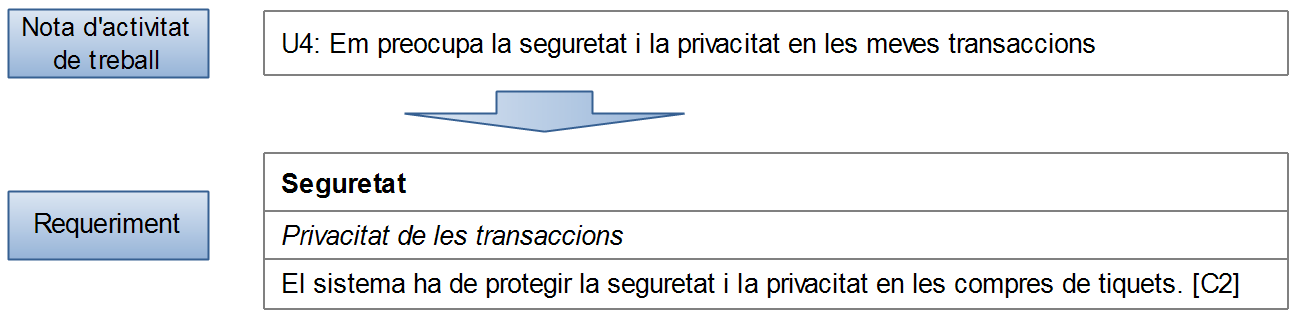
\includegraphics[scale=0.3]{WorkActivityNotes2.png}
\caption{Documents resultants de l'extracció de requeriments}\label{fig:workActivityNote2}
\end{figure}

A la figura \ref{fig:workActivityNote2} es pot veure com s'extreu un requeriment, utilitzant el mateix exemple que abans (figura \ref{fig:workActivityNote1}). L'etiqueta "C2", fa referencia a la posició que ocupava la nota dins el \ac{WAAD}. S'utilitzen les lletres per anomenar les diferents branques i sub-branques i els números per diferenciar les notes que hi ha la mateixa branca del \ac{WAAD}.

Un cop generats els requeriments es comprovarà que aquests siguin correctes preguntant directament als usuaris. Sempre que sigui possible es preguntarà als usuaris que van participar en la investigació contextual (apartat \ref{subsec:investigacio_contextual} juntament amb d'altres nous usuaris. Aquest pas també pot servir perquè els usuaris ajudin a destacar aquells requeriments que són prioritaris.

\subsubsection{Construcció de models informatius per al disseny}\label{subsubsec:Construccio_models}
Per dur a terme aquesta etapa també cal recórrer el \ac{WAAD}, és per això que aquesta etapa no és posterior a l'etapa \ref{subsubsec:Extraccio_requeriments} sinó que les dues es duen a terme de forma paral·lela. L'objectiu d'aquesta etapa és obtenir una sèrie de documents que descriuen tant el sistema actual, com el sistema que es preveu. Aquests documents seran els que es faran servir per a dissenyar el nou producte.

Aquest pas, juntament amb l'anterior (apartat \ref{subsec:analisi_contextual}) serveixen de pont entre l'anàlisi en si i l'etapa del disseny. És a dir, serveixen per enllaçar la situació o model actual, amb el model o sistema que s'està dissenyant.

Els documents que s'obtenen en aquesta etapa (figura \ref{fig:design-informing_models}) són: 
\begin{figure}[ht]
\centering
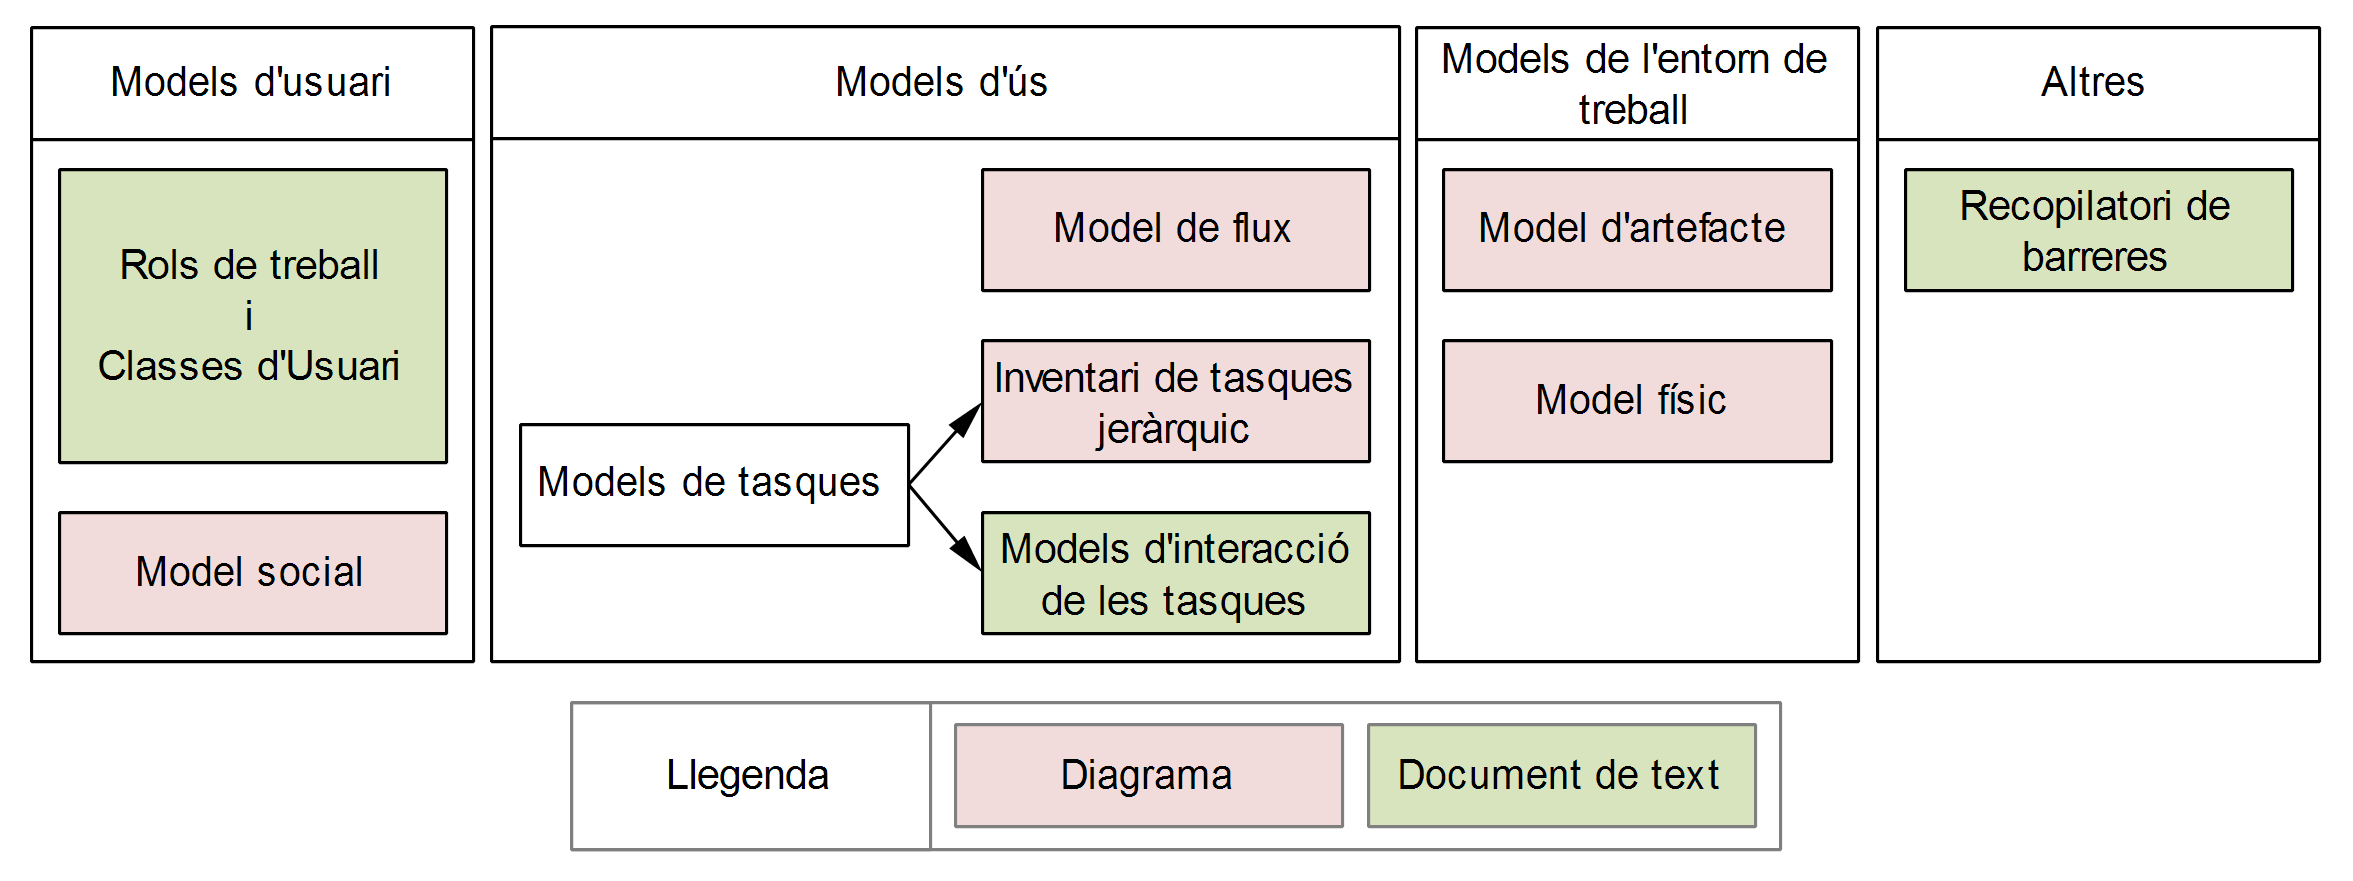
\includegraphics[scale=0.75]{Design-informing_models.png}
\caption{Exemple d'extracció de requeriments}\label{fig:design-informing_models}
\end{figure}

\begin{description}
\item[Rols de treball] Corresponen als deures, funcions i activitats que desenvolupa una persona amb cert lloc de treball.
\item[Classes d'Usuaris] Són les diferents característiques de la gent que desenvolupa un rol de treball concret.
\item[Model social] És un diagrama que mostra l'organització i relació que existeix entre les diferents persones que intervenen en el sistema.
\item[Model de flux] Aquest diagrama mostra com les diferents entitats (ja siguin, persones, aparells o programes) interaccionen entre si i què intercanvien entre elles.
\item[Inventari de tasques jeràrquic] Es tracta d'un inventari jeràrquic que mostra les diferents tasques que es poden executar en el sistema.
\item[Models d'interacció de les tasques] És un document que detalla com es duen a terme les tasques i com interaccionen les entitats que intervenen (sempre que intervingui més d'una entitat).
\item[Model d'artefacte] Aquest diagrama mostra com els diferents elements tangibles interactuen entre si.
\item[Model físic] Aquest model mostra la distribució física dels diferents artefactes i entitats.
\item[Recopilatori de barreres] És un recopilatori de les barreres que s'han descrit als documents anteriors.
\end{description}

Una barrera és un problema que interfereix amb les operacions que l'usuari executa normalment. És qualsevol cosa que impedeix l'activitat de l'usuari, interromp el flux habitual del treball o interfereix amb el desenvolupament del treball. Seguint les recomanacions de Rex Harton (2012, p. 186) \cite{UX_Book} habitualment s'utilitza la mateixa simbologia que Beyer i Holtzblatt \cite{Contextual_Design} per a representar les barreres (el llamp vermell \barrier)

\subsection{Disseny}
Aquest pas consisteix en crear diversos dissenys conceptuals que mostren com serà el producte que es busca crear, determinant com ha de ser la interacció amb aquest i la seva aparença. 

Al dissenyar és important saber per a quin tipus d'usuari es dissenya. I és que tal com diu Cooper (2004, p. 124) \cite{Cooper} no és possible crear un disseny que funcioni per a tothom i és millor tenir un petit percentatge de la població completament satisfeta que no pas tota la població mig satisfeta. Afirma que fins i tot és preferible tenir un percentatge més petit de la població extasiada amb el producte. Per a facilitar que en aquesta etapa es dissenyi per a satisfer totes les necessitats de cert grup de la població, cal crear personatges, creant un personatge per a cada rol definit prèviament. La creació d'aquests personatges és un pas clau per a aconseguir crear un bon producte. Per a crear cada personatge primer es creen personatges a partir dels usuaris que han intervingut a l'anàlisi. Després es fusionen els personatges que tenen les mateixes metes. Ara, d'entre els personatges que queden, cal escollir aquell personatge que, si es dissenya exclusivament per a ell, el producte funcionarà prou bé per la resta de persones. Si cal s'agafaran característiques de diferents personatges per a crear el personatge definitiu. 

Un cop es tenen els personatges creats, comença la part del disseny en si. Aquí Rex (2012, p. 335) \cite{UX_Book} proposa fer 5 passos on cada cop es refina més el disseny, fins a assolir el disseny definitiu. Aquestes etapes són:

\begin{itemize}
\item Ideació i esbossos
\item Disseny conceptual
\item Disseny intermedi
\item Disseny detallat
\item Refinat del disseny
\end{itemize}


\subsubsection{Ideació i esbossos}
Aquest primer pas consisteix en explorar idees. Per una banda amb la ideació, és a dir, el procés de formar idees per el disseny, la qual cosa normalment és fa amb una pluja d'idees. Per l'altre es creen esbossos per a plasmar les idees d'alguna de les persones que està dissenyant. Es important remarcar que les idees o esbossos que es creen en aquest pas han de tenir un nivell de detall molt baix. El que es busca és un primer contacte amb les idees, per tant és important deixa llibertat per a que sorgeixin el màxim d'idees, sense limitar-les a si semblen factibles o no. 

\subsubsection{Disseny conceptual}
Per \gls{conceptual_design} s'entén, un tema, noció o idea amb el propòsit de comunicar una visió del disseny del sistema o producte. És la part del disseny del sistema que porta el model mental del dissenyador a la vida. 
Aquí es busca avaluar i comparar diversos dissenys conceptuals mirant també la seva viabilitat. 

\subsubsection{Disseny intermedi}
L'objectiu del disseny intermedi és crear la navegació, estructura i disseny de les pantalles, amb un nivell de fidelitat mitjà. Parteix dels dissenys conceptuals i es busca descomposar-los en unitats lògiques, expandint-les en diferents possibilitats de disseny. 

En el disseny intermedi és defineix completament com ha de ser la navegació. Tot i això el contingut de cada apartat o pàgina només es mostra de forma aproximada, amb un nivell de fidelitat mitjà, sense masses detalls. 
És en aquesta etapa on prenen màxima rellevància els documents que s'han obtingut en l'etapa de construcció de models informatius \ref{subsubsec:Construccio_models}.

\subsubsection{Disseny detallat}
En aquest pas es busca detallar el disseny. Aquí es defineix completament l'aparença de tots els elements que apareixen en pantalla, definint els objectes que els formen, colors, mides, fonts, marges i localització de cada un d'ells. A la figura \ref{fig:design_Sunshine} es pot veure un exemple de disseny detallat d'una aplicació per \gls{Android}.

\begin{figure}[ht]
\centering
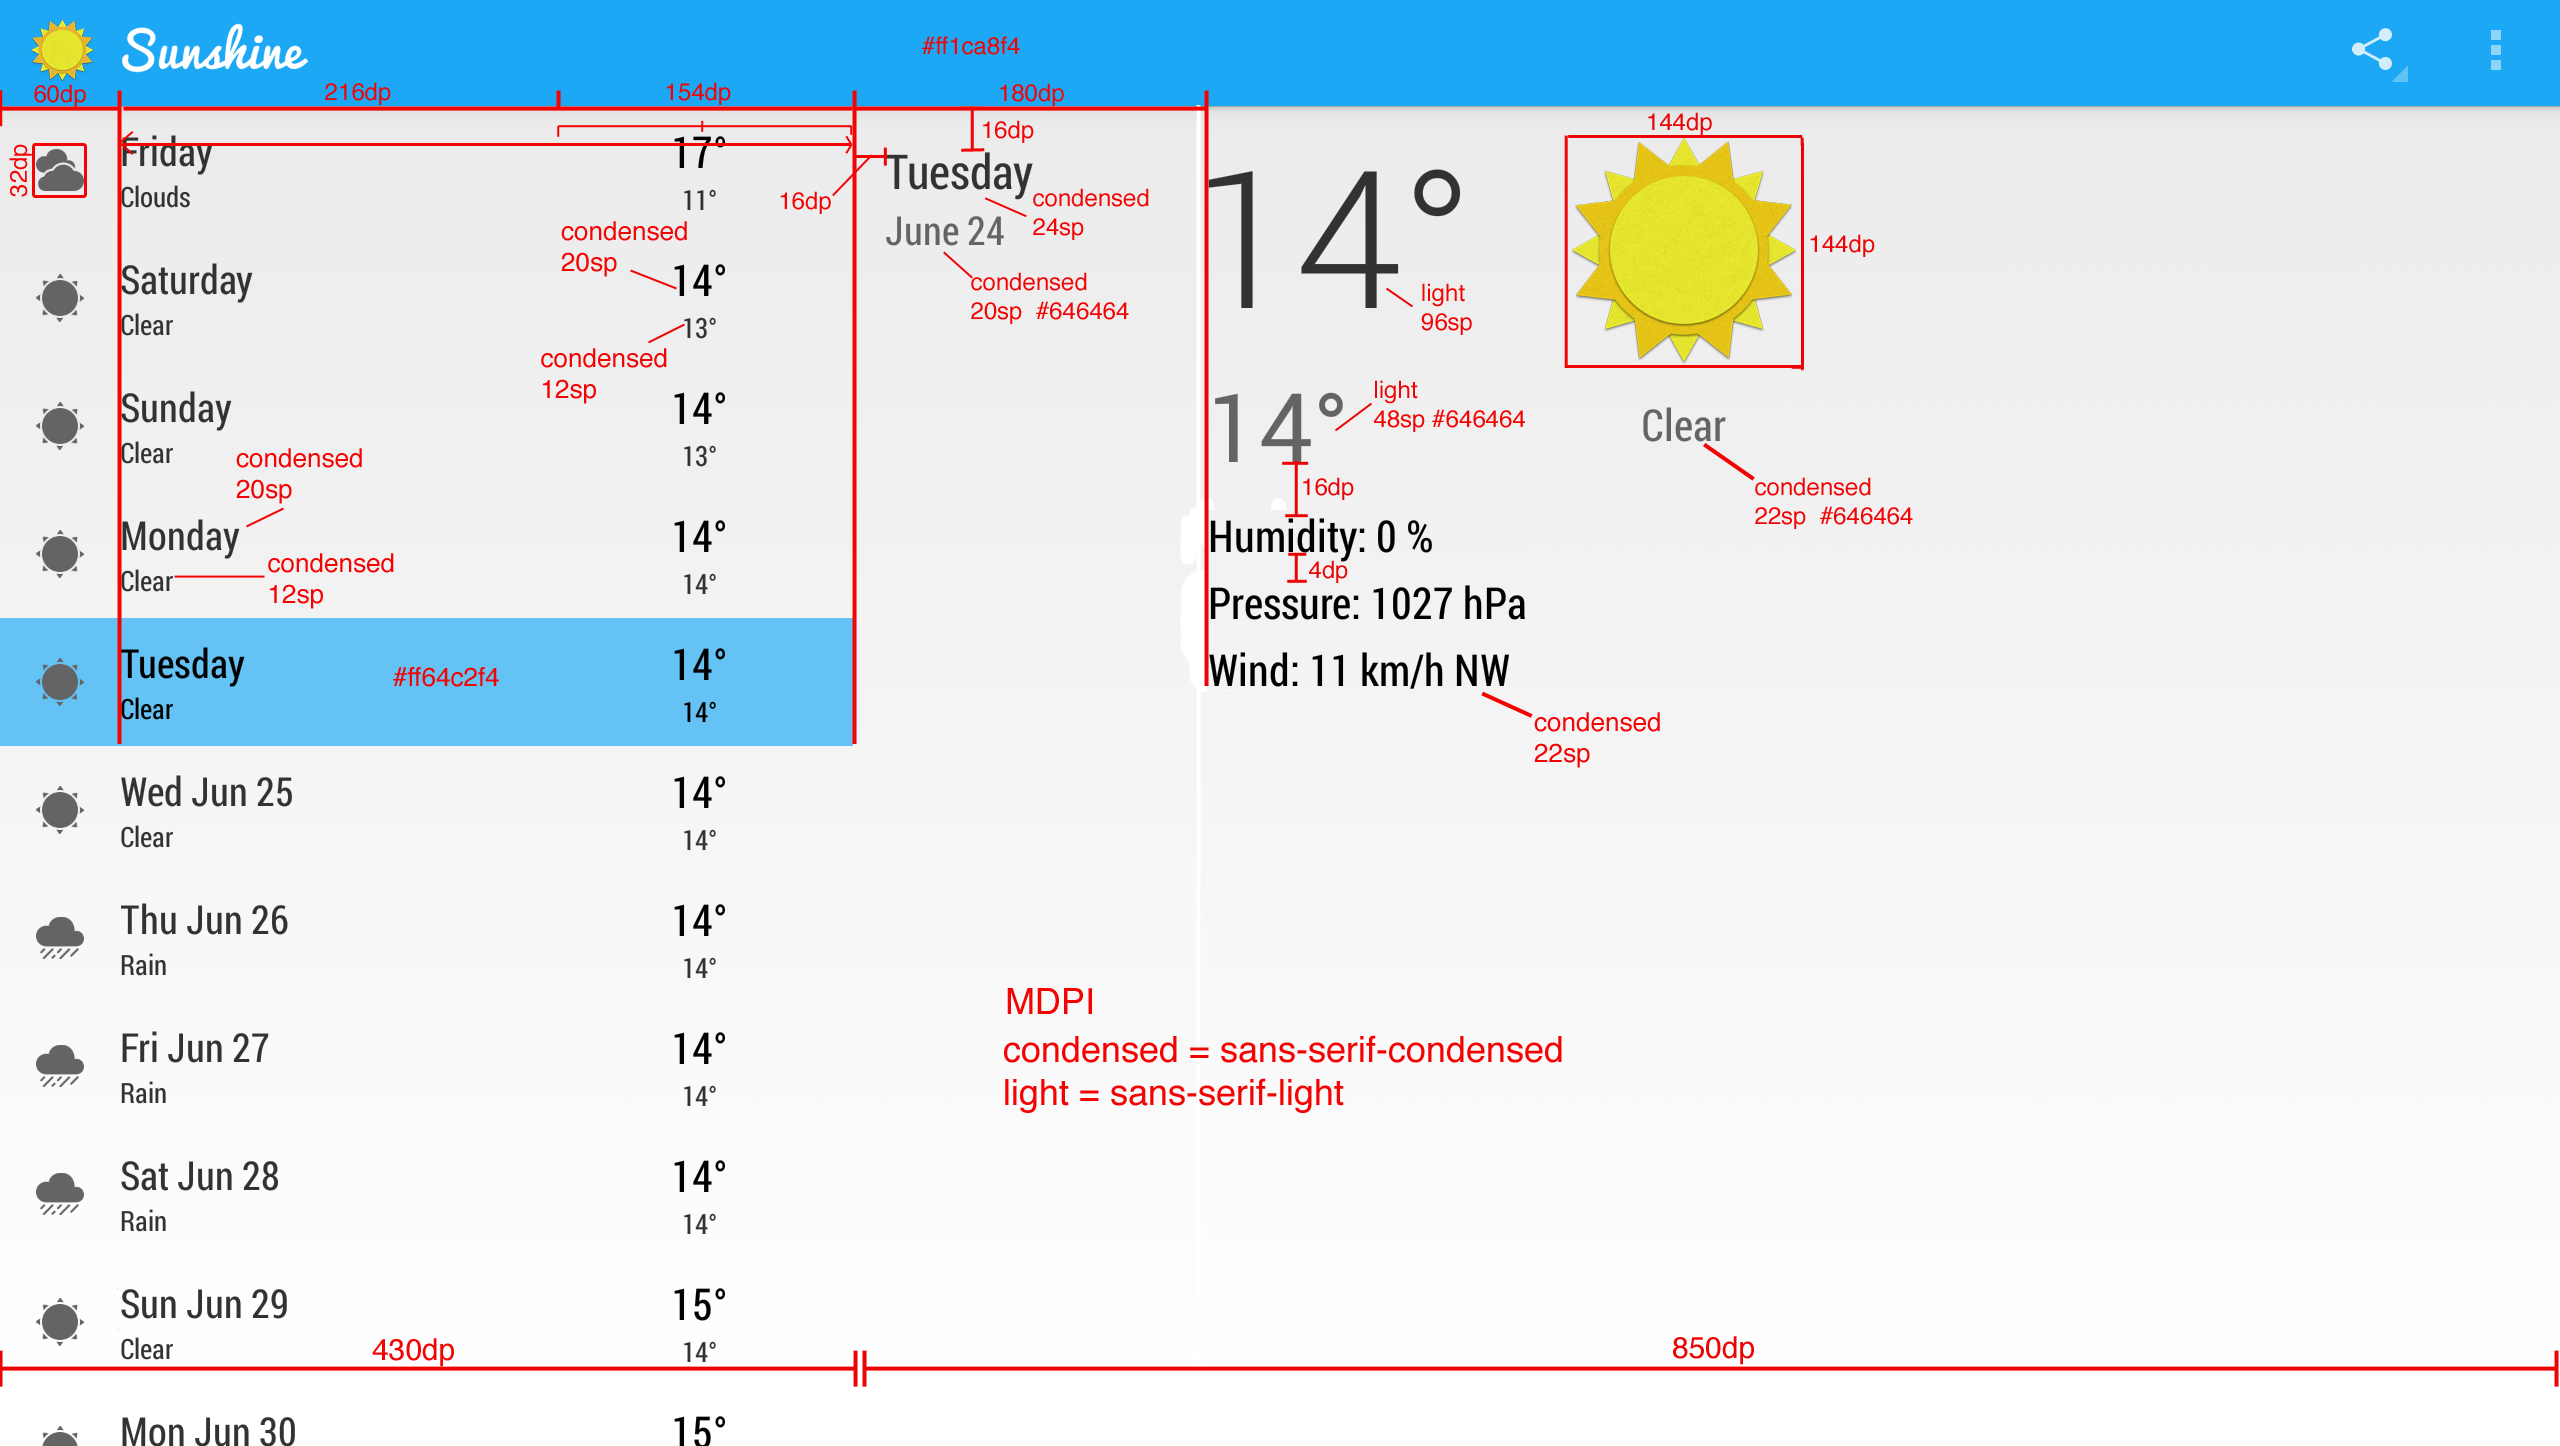
\includegraphics[scale=0.17]{Sunshine_detailed_design.png}
\caption{Exemple de disseny detallat. Font: Udacity (Developing Android Apps) \cite{developing_android_apps}}
\label{fig:design_Sunshine}
\end{figure}

\subsubsection{Refinat del disseny}
Aquesta etapa es centra a buscar i arreglar problemes de \ac{UX} 


%TODO HEX proposa que s'adaptin els metodes als recursos disponibles
\subsection{Implementació}\label{subsec:implementation}
En la implementació o prototipatge es busca poder avaluar amb els usuaris els dissenys que s'han creat i es du a terme mitjançant prototips, els quals són representacions navegables del producte final. Tal com Nielsen (1993) \cite{Nielsen_1993} proposa, els prototips es poden classificar segons la funcionalitat i segons les funcions o característiques que implementen, tal com es veu a la figura \ref{fig:types_prototypes}. També defineix els prototips horitzontals, verticals i locals. Aquests es caracteritzen per:

\begin{figure}[ht]
\centering
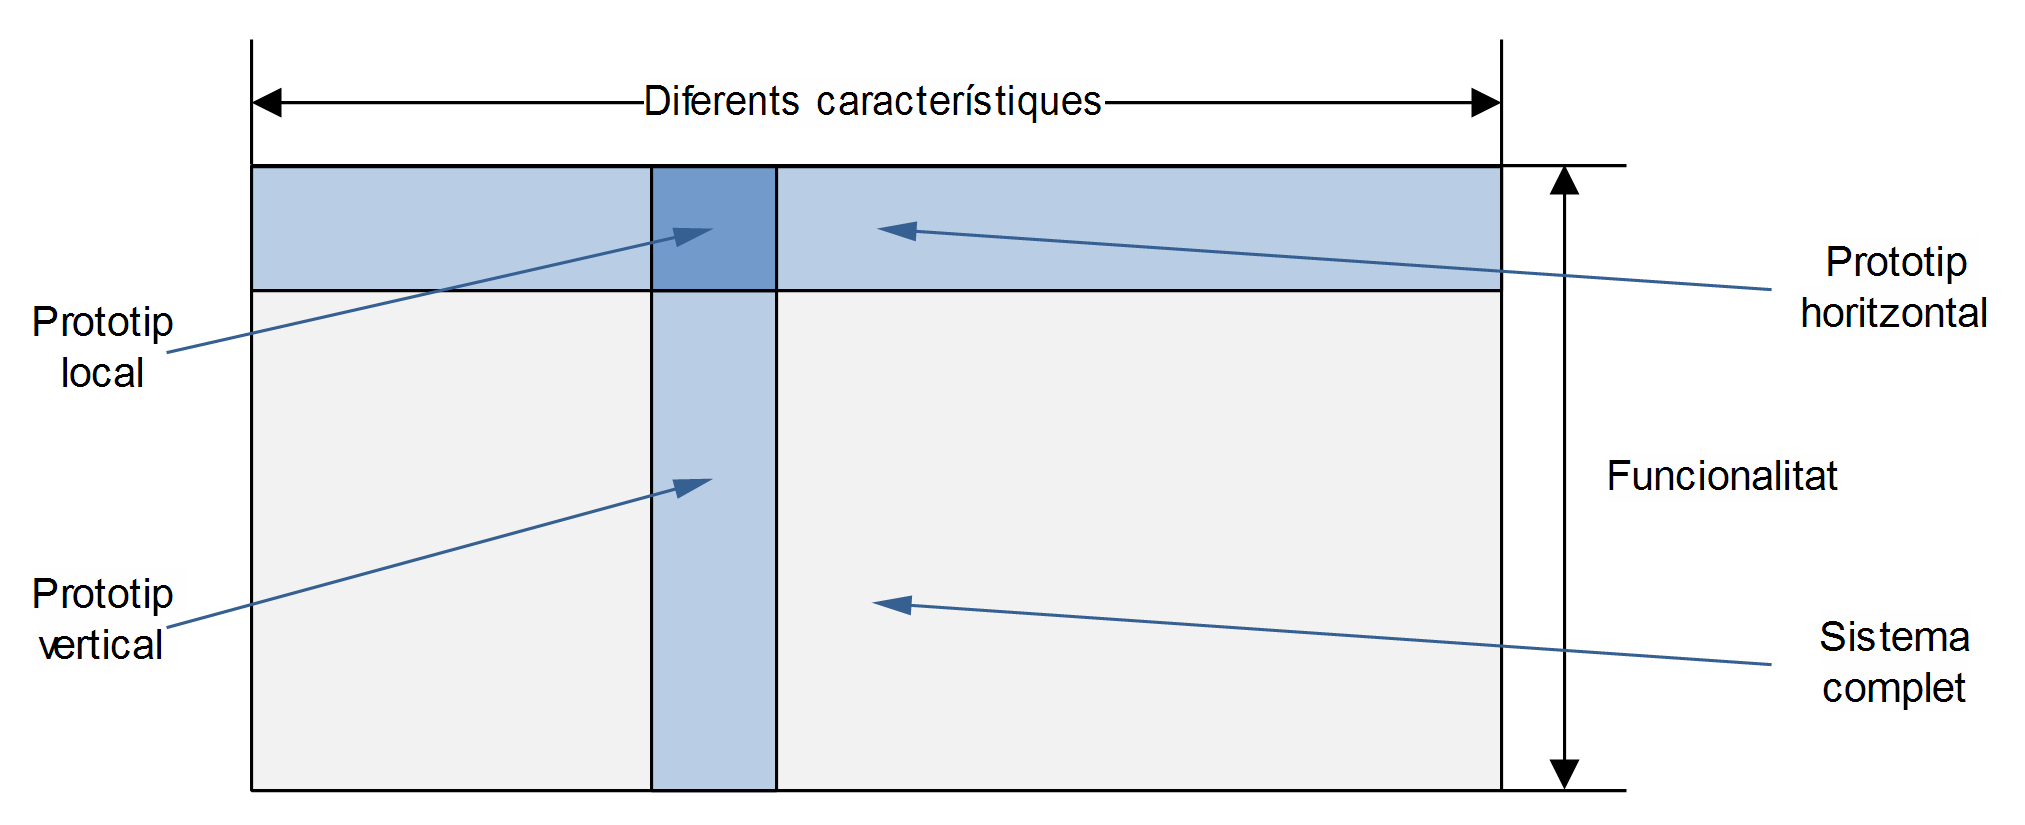
\includegraphics[scale=0.8]{Types_prototypes.png}
\caption{Tipus de prototips}\label{fig:types_prototypes}
\end{figure}

\begin{description}
\item[Prototip Horitzontal] És caracteritza per tenir moltes funcions però amb una profunditat molt baixa de funcionalitat. Serveix per a demostrar les diferents característiques o funcions que tindrà el producte, de manera que es pot veure de forma general les seccions o apartats i la navegació en general.
\item[Prototip Vertical] Aquest tipus de prototip té una profunditat màxima de funcionalitat però centrat només en unes poques funcions. S'utilitza per avaluar amb suficient detall algunes funcions concretes del producte. 
\item[Prototip Local] És un tipus de prototip on només implementa unes poques funcions i amb poca profunditat en quan a funcionalitat. S'utilitzen per avaluar diferents alternatives de disseny per a certs detalls d'interacció amb el sistema. 
\end{description}

Els prototips també es poden classificar segons el nivell de fidelitat, és a dir, com de "finalitzat" percep l'usuari el prototip. Es classifiquen doncs en baixa, mitja o alta fidelitat. 

\begin{description}
\item[Prototips de baixa fidelitat] Aquests prototips s'utilitzen en les primeres etapes de disseny, ja que impliquen poca feina i per tant són senzills de modificar. Aquest tipus de prototips habitualment es fan dibuixant amb paper i bolígraf. 
\item[Prototips de mitja fidelitat] Es tracta d'un terme mig entre prototip de baixa i el d'alta fidelitat. Tot i que no representen l'aspecte final del producte, si s'acosten donant una idea més real de com serà. Aquests tipus de prototips normalment es creen amb programes especials per a ordinadors.
\item[Prototips d'alta fidelitat] Els prototips d'alta fidelitat tenen un aspecte i comportament molt realista i pròxim al producte final. S'utilitzen per a polir i refinar el disseny del producte. 
\end{description}

Quan menys fidel és un prototip, és alhora més susceptible de canviar. I és que un prototip de baixa fidelitat és percebut com a poc fidel al producte final per un usuari, i com a conseqüència, desinhibeix als usuaris a l'hora de criticar-lo i aportar idees per a millorar-lo. En canvi, en un prototip d'alta fidelitat, al ser tant pròxim al producte final, l'usuari percep que hi ha molta feina darrere d'aquest i que per tant és complicat modificar-lo i això portarà a que tendeixi a no criticar-lo, amb la idea de no menystenir la feina d'altres persones. Tot i això, els prototips de baixa fidelitat són complicats d'entendre per les persones que no estan familiaritzades, per això és recomanable que només s'utilitzin i es comparteixin amb l'equip de disseny i, si existeixen, amb usuaris que estiguin familiaritzats amb el procés de disseny. Per tant, de forma general, els prototips de mitja fidelitat són els primers que es comparteixen amb els usuaris. 


Els prototips són representacions navegables que exemplifiquen com serà el producte o sistema. Com a tals, hi ha varies maneres d'aconseguir que siguin navegables, permetent més o menys interacció. Es tenen doncs:

\begin{description}
\item[Prototips de paper] Consisteix en crear en paper els diferents elements del sistema i utilitzar una base per a poder-los mostrar. L'usuari simula clics als diferents elements i l'avaluador far aparèixer els elements necessaris que corresponen a la resposta del clic que ha fet l'usuari. 
\item[Prototips "Mag d'Oz"] Aquests tipus de prototips es basen en dos aparells, un per a l'usuari i un per l'avaluador. L'usuari interactuarà amb el seu dispositiu i l'avaluador, amb l'altre dispositiu rebrà les accions de l'usuari i les respondrà simulant el comportament del sistema.
\item[Prototip completament programat] És un prototip programat que representa de manera bastant fidel el producte/sistema final.
\end{description}

Durant la creació d'un producte el més habitual és començar creant prototips horitzontals de baixa fidelitat per a poder generar una primera impressió del producte. A mesura que es va perfeccionant el producte, es va millorant la fidelitat d'aquest i permetent més interacció de manera que els usuaris notin que interactuen amb prototip molt semblant al producte final. D'aquesta manera s'inverteixen pocs recursos amb els primers prototips ja que són més susceptibles de canviar i un cop es sap que el producte va per el bon camí es quan es creen els prototips d'alta fidelitat, invertint només una quantitat elevada de recursos quan és necessari. 

\subsection{Avaluació}
Per avaluació s'entén validar que el producte compleix les expectatives dels usuaris. Per a fer-ho, hi ha dos tipus d'avaluació, l'avaluació formativa i la sumarial. 

\begin{description}
\item[Avaluació formativa] Es tracta d'un primer diagnostic. Consisteix en recol·lectar informació qualitativa per identificar i arreglar problemes de \ac{UX} i les seves causes en el disseny.
\item[Avaluació sumarial] Consisteix en recol·lectar informació quantitativa per assegurar un nivell de qualitat en un disseny, especialment per a l'avaluació de la millora de la \ac{UX} a causa de l'avaluació formativa. Es dur a terme en les últimes fases de disseny quan els prototips ja tenen una fidelitat alta. 
\end{description}

La informació que s'obté a l'avaluació pot ser objectiva o subjectiva i quantitativa o qualitativa.

\begin{description}
\item[Informació objectiva] Es tracta d'informació observada per l'avaluador o per l'usuari sobre inconsistències o problemes. 
\item[Informació subjectiva] Són les opinions o judicis del usuaris respecte a la seva \ac{UX} i la satisfacció al interactuar amb el producte. 
\item[Informació quantitativa] És la informació numèrica que demostra la qualitat del producte. S'obté a través d'analitzar el rendiment o amb qüestionaris i és la base de l'avaluació sumarial.
\item[Informació qualitativa] És informació descriptiva que normalment descriu problemes d'\ac{UX} observats durant la utilització del producte.
\end{description}

Per a poder recopilar informació a l'hora d'avaluar, Rex (2012, p. 360 - 490) \cite{UX_Book} proposa un seguit de tècniques:

\begin{itemize}
\item Detecció d'incidents crítics
\item Tècnica "pensar en veu alta"
\item Demostració del producte
\item Inspecció 
\item Qüestionaris
\item Versions alfa/beta
\item Mètriques \ac{UX}
\end{itemize}

\subsubsection{Detecció d'incidents crítics}
Un incident crític és un esdeveniment observat durant el desenvolupament de les tasques que ha produït sorpresa, ha molestat o inquietat a l'usuari per la seva falta de coherència o per presentar resultats inesperats per l'usuari. La detecció d'incidents crítics consisteix en analitzar els usuaris mentre utilitzen el producte per a poder trobar-los. És una tècnica d'avaluació formativa que serveix per a recopilar informació qualitativa. Els incidents crítics sovint són expressats verbalment per els usuaris, però a vegades també poden ser expressats de forma no verbal mitjançant unt titubeig, encongiment d'espatlles o alguna ganyota. 
\subsubsection{Tècnica "pensar en veu alta"}
La tècnica "pensar en veu alta" és una tècnica per aconseguir informació qualitativa que, com el seu nom indica, consisteix en què el usuaris expressin verbalment els seus pensaments, els seus motius i la seva percepció sobre els problemes d'\ac{UX} en quan a la interacció amb el producte quan l'estan fent servir. Amb aquesta tècnica s'aconsegueix entendre que és el que l'usuari intenta fer en tot moment i quins problemes experimenta.
És important que els usuaris expliquin què és el que estan pensant, no el que estan fent, ja que això és el que seria més complicat de saber sense fer servir aquesta tècnica.  
\subsubsection{Demostració del producte}
Una demostració o \textit{walkthrough} és un mètode que s'acostuma a fer servir en les primeres etapes de disseny abans que existeixi algun prototip. Consisteix en ensenyar el producte als usuaris fent-se passar per un, de manera que aquests veuran el disseny com si fossin uns experts. La idea és que l'equip intenta anticipar-se als problemes que els usuaris podrien tenir si fossin ells els que estiguessin utilitzant el producte. 
\subsubsection{Inspecció} 
La inspecció consisteix en que un expert en UX provi i avaluï ell mateix el producte enlloc de que el facin servir usuaris mentre l'expert els observa. Per tant, l'avaluador fa alhora d'observador i participant. Aquesta tècnica és útil a les primeres etapes del disseny per a poder trobar els problemes d'\ac{UX} més evidents a un baix cost. 
\subsubsection{Qüestionaris}
Els qüestionaris són la eina principal per a recol·lectar informació objectiva del producte. S'utilitzen principalment com a una eina de formació sumarial. Hi ha molts qüestionaris creats específicament per avaluar l'\ac{UX}, tot i això els més coneguts i d'ús lliure són:
\begin{itemize}
\item Qüestionari per a la satisfacció amb la interfície d'usuari o \textit{Questionnaire for User Interface Satisfaction} (QUIS).
\item Escala d'usabilitat del sistema o \textit{System Usability Scale} (SUS).
\item Utilitat, satisfacció i facilitat d'ús o \textit{Usefulness, Satisfaction and Ease of Use} (USE).
\end{itemize}

\subsubsection{Versions alfa/beta}
Quan el producte és una aplicació de \textit{software} i el procés de desenvolupar-la s'ha acabat és habitual que s'envii primer a certs usuaris, experts, clients i crítics professionals per a que en donin la seva opinió. Una versió alfa és una versió més prematura i menys polida del producte que s'envia a una audiència més reduïda també a l'objectiu d'aconseguir la seva opinió. 
Aquestes versions són una forma gratuïta d'aconseguir les opinions dels usuaris abans de llançar finalment el producte al mercat i serveixen per a comprovar com acollirà el públic el producte. Sovint també serveix per a detectar erros que s'hagin pogut passar per alt al desenvolupar el producte. 

\subsubsection{Mètriques \ac{UX}}
Aquesta tècnica consisteix en establir certs objectius en quan a \ac{UX} que siguin quantificables. Un cop establits, es defineix un valor mínim o cota, normalment amb un producte ja existent. Quan ja es té un valor es tracta de calcular el valor de cada mètrica amb el prototip i veure si és supera la cota. En aquesta tècnica es fan servir les taules de mètriques com per exemple la taula \ref{table:UX_metrics}.

\begin{table}
\begin{tabular}{ | p{2.4cm} | p{2.7cm} | p{2.6cm} | p{1.6cm} | p{2.6cm} |}
\hline
\headB{Objectiu \ac{UX}} & \headB{Mesura \ac{UX}} & \headB{Mètrica \ac{UX}} & \headB{Cota} & \headB{Valor observat} \\
\hline
Facilitat d'ús & Rendiment inicial de l'usuari & Temps mitjà & 3 min. & 2,5 min. \\
\hline
Facilitat d'ús & Rendiment inicial de l'usuari & Nombre mitjà d'errors & $<1$ & $<1$ \\
\hline
\end{tabular}
\caption{Taula exemple de les mètriques \ac{UX}}
\label{table:UX_metrics}
\end{table}


\section{El procés iteratiu}
A l'hora de dissenyar per a una bona \ac{UX} és important fer les quatre activitats fonamentals de forma iterativa per tal d'assegurar que la solució realment és bona. Per tant, quan és fa un estudi d'\ac{UX} és comença amb un anàlisi utilitzant els productes/sistemes semblants al que es vol dissenyar per a veure com els usuaris interactuen amb ell i que n'esperen. Un cop finalitzada l'etapa de l'anàlisi per primer cop, és faran els primers dissenys i s'implementaran fent els primers prototips de baixa fidelitat per no malbaratar recursos. Amb aquests prototips s'avaluarà la idoneïtat de la solució dissenyada i, si s'escau, és corregiran els documents que s'havien aconseguit a l'etapa de l'anàlisi. Un cop s'ha fet la primera iteració, s'anirà fent dissenys cada cop més detallats i implementant prototips de fidelitat més alta. D'aquesta manera s'acabarà arribant a un disseny definitiu i a un prototip que serà molt semblant a com ha de ser el producte final.

Al ser un procés iteratiu pot semblar que a les primeres iteracions no és imprescindible arribà a un disseny i/o prototip bo, ja que en les següents iteracions ja s'aconseguirà que aquests siguin bons. Però a la realitat això no és així, cada iteració implica utilitzar recursos, per tant per a ser eficients és millor no fer masses iteracions. És a dir, des d'un bon principi és busca aconseguir dissenyar garantint la millor \ac{UX} possible.

A la taula \ref{table:UX_sum_up} és mostra un resum aproximat de com és relacionen les diferents etapes entre si. És una representació dels passos que es segueixen durant el procés iteratiu. Tot i que s'ha intentat ordenar cronològicament en funció de l'ordre d'execució, a la realitat és habitual que algunes etapes es solapin o es duguin a terme simultaneïtat, sobretot quan s'estan explorant diversos possibles dissenys.

\begin{table}
\begin{tabular}{ | p{1.8cm} | p{5cm} | p{3cm} | p{3cm} |}
\hline
\headB{Passos del disseny} & \headB{Propòsit} & \headB{Prototip} & \headB{Avaluació} \\
\hline
Ideació i esbossos & Explorar idees de disseny & Esbossos & Discutint i criticant amb l'equip de disseny \\
\hline
Disseny conceptual & Avaluar i comprar múltiples dissenys conceptuals & Prototips de paper i \gls{wireframe} i \textit{storyboards} de baixa fidelitat &  Fent demostracions del producte als equips de treball involucrats amb el producte\\ 
\hline
Disseny intermedi & Filtrar els dissenys conceptuals, tot definint la navegació, fins a arribar al disseny conceptual definitiu & \textit{wireframes} d'alta o mitja fidelitat & Validar amb els usuaris (Avaluació formativa)\\
\hline
Disseny detallat & Definir completament el disseny, definint amb detall l'aparença, la distribució i comportament de les pantalles & \textit{wireframes} d'alta fidelitat i maquetes o prototips interactius & Validar amb els usuaris (Avaluació formativa)\\
\hline
Refinat del disseny & Avaluar el disseny final alhora que trobar i eliminar el màxim de problemes de \ac{UX} & Prototip programat d'alta fidelitat& Validar amb els usuaris (Avaluació sumarial) \\
\hline
\end{tabular}
\caption{Relacions entre les diverses etapes en un estudi d'\ac{UX}}
\label{table:UX_sum_up}
\end{table}
\chapter{Estat de l'art}
\section{Aplicacions existents}
En quan a les aplicacions que es poden trobar actualment a \gls{Google_play}, la botiga virtual d'aplicacions per \gls{Android}, existeixen moltes que serveixen per a la gestió de despeses. És per això que s'estudiaran només les més rellevants i representatives, les quals tenen un mínim de 100.000 descarregues. Les aplicacions que s'han tingut en compte són les de la taula (\ref{fig:apps}). 

\begin{table}
\begin{tabular}{ | l | c | l | l | }
\hline
\textbf{Núm.} & \textbf{Icona} & \textbf{Nom} & \textbf{Autor} \\
\hline
App 1 & 
\includegraphics[scale=0.05]{A01_icon.png} & \href{https://play.google.com/store/apps/details?id=com.expensemanager}{Expense Manager} & Bishinews \\

App 2 & 
\includegraphics[scale=0.05]{A02_icon.png} & \href{https://play.google.com/store/apps/details?id=at.markushi.expensemanager}{Expense Manager} & Markus Hintersteiner \\

App 3 & 
\includegraphics[scale=0.05]{A03_icon.png} & \href{https://play.google.com/store/apps/details?id=com.bruno.myapps.droidwallet}{Droid Wallet} & William Bruno \\

App 4 & 
\includegraphics[scale=0.05]{A04_icon.png} & \href{https://play.google.com/store/apps/details?id=com.code44.finance}{Financius - Expense Manager} & Mantas Varnagiris \\

App 5 & 
\includegraphics[scale=0.05]{A05_icon.png} & \href{https://play.google.com/store/apps/details?id=com.handyapps.expenseiq}{Expense IQ} & Handy Apps \\

App 6 & 
\includegraphics[scale=0.05]{A06_icon.png} & \href{https://play.google.com/store/apps/details?id=com.techahead.ExpenseManager}{Diario Gasto Gerente (Daily Expense Manager)} & Gullak \\

App 7 & 
\includegraphics[scale=0.05]{A07_icon.png} & \href{https://play.google.com/store/apps/details?id=com.bookmark.money}{Money lover - Expense Manager} & ZooStudio   \\

App 8 & 
\includegraphics[scale=0.05]{A08_icon.png} & \href{https://play.google.com/store/apps/details?id=com.kpmoney.android}{AndroMoney (Expense Track)} & AndroMoney \\

App 9 & 
\includegraphics[scale=0.05]{A10_icon.png} & \href{https://play.google.com/store/apps/details?id=cz.destil.settleup}{Settle up} & David Vávra \\

App 10 & 
\includegraphics[scale=0.05]{A11_icon.png} & \href{https://play.google.com/store/apps/details?id=com.Splitwise.SplitwiseMobile}{Splitwise} & Splitwise \\

\hline
\end{tabular} 
\caption{Taula amb les aplicacions existents}
\label{fig:apps}
\end{table}

Actualment hi ha dos tipus d'aplicacions relacionades amb la gestió de despeses. Per una banda les que serveixen per enregistrar les despeses i/o ingressos personals, tot categoritzant-los (Aplicacions 1 - 8) i per l'altra les que serveixen per a gestionar despeses compartides en grup i/o deutes personals amb coneguts (Aplicacions 9 i 10).

%TODO More info about SUS. 
Per a veure el grau de satisfacció dels usuaris amb les aplicacions existents s'ha fet servir el qüestionari \gls{SUS} amb 4 usuaris. Amb els resultats s'ha fet la mitjana dels 4 usuaris per cada aplicació donant com a resultat els valors de la figura (\ref{fig:Apps_art_state}). Com es pot veure els usuaris no tenen una bona \ac{UX} al fer servir varies d'aquestes aplicacions, ja que obtenen una nota bastant baixa.

\begin{figure}[htp]
\centering
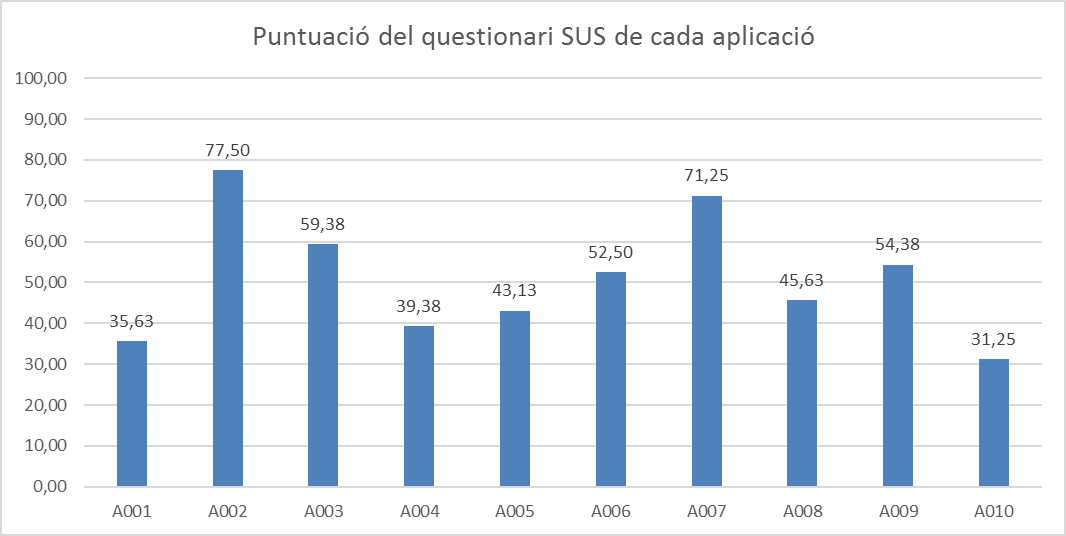
\includegraphics[scale=0.8]{Apps_art_state_SUS.png}
\caption{Puntuació de les aplicacions existents amb el questionari SUS}\label{fig:Apps_art_state}
\end{figure}

\subsection{Aplicacions per gestionar despeses en grup}



\include{20_estudi}
\chapter{Avaluació dels resultats}
\chapter{Disseny de l'aplicació}
Tot i que el disseny en general de l'aplicació no és rellevant per aquest projecte, si que es considera important destacar algunes parts d'aquesta, concretament el disseny de la base de dades i la resolució del problema del repartiment de despeses en grup.

%TODO link codi


\section{Disseny de la base de dades}
A l'hora d'emmagatzemar les dades de la aplicació s'ha optat per fer servir \gls{SQLite} de forma local al \gls{smartphone} i fer ús del \gls{BAAS} Parse.com. Per tant s'ha dissenyat una base de dades local i una altre al núvol. La base de dades principal és la local i la del núvol està com a còpia de seguretat i per garantir la sincronització multidispositiu. Les taules que han de ser llegides per varies persones s'han partir en dues, una privada i una pública, al emmagatzemar-les al núvol de manera que el mínim d'informació és accessible per als usuaris que no l'han creat.

A la figura \ref{fig:db_sqlite} es pot veure el disseny de la base de dades local, a la figura \ref{fig:db_parse} es pot veure la base de dades al núvol i a la figura \ref{fig:db_private_shared} és pot veure quines columnes són privades i quines públiques a cada taula. 

\begin{figure}[ht]
\centering
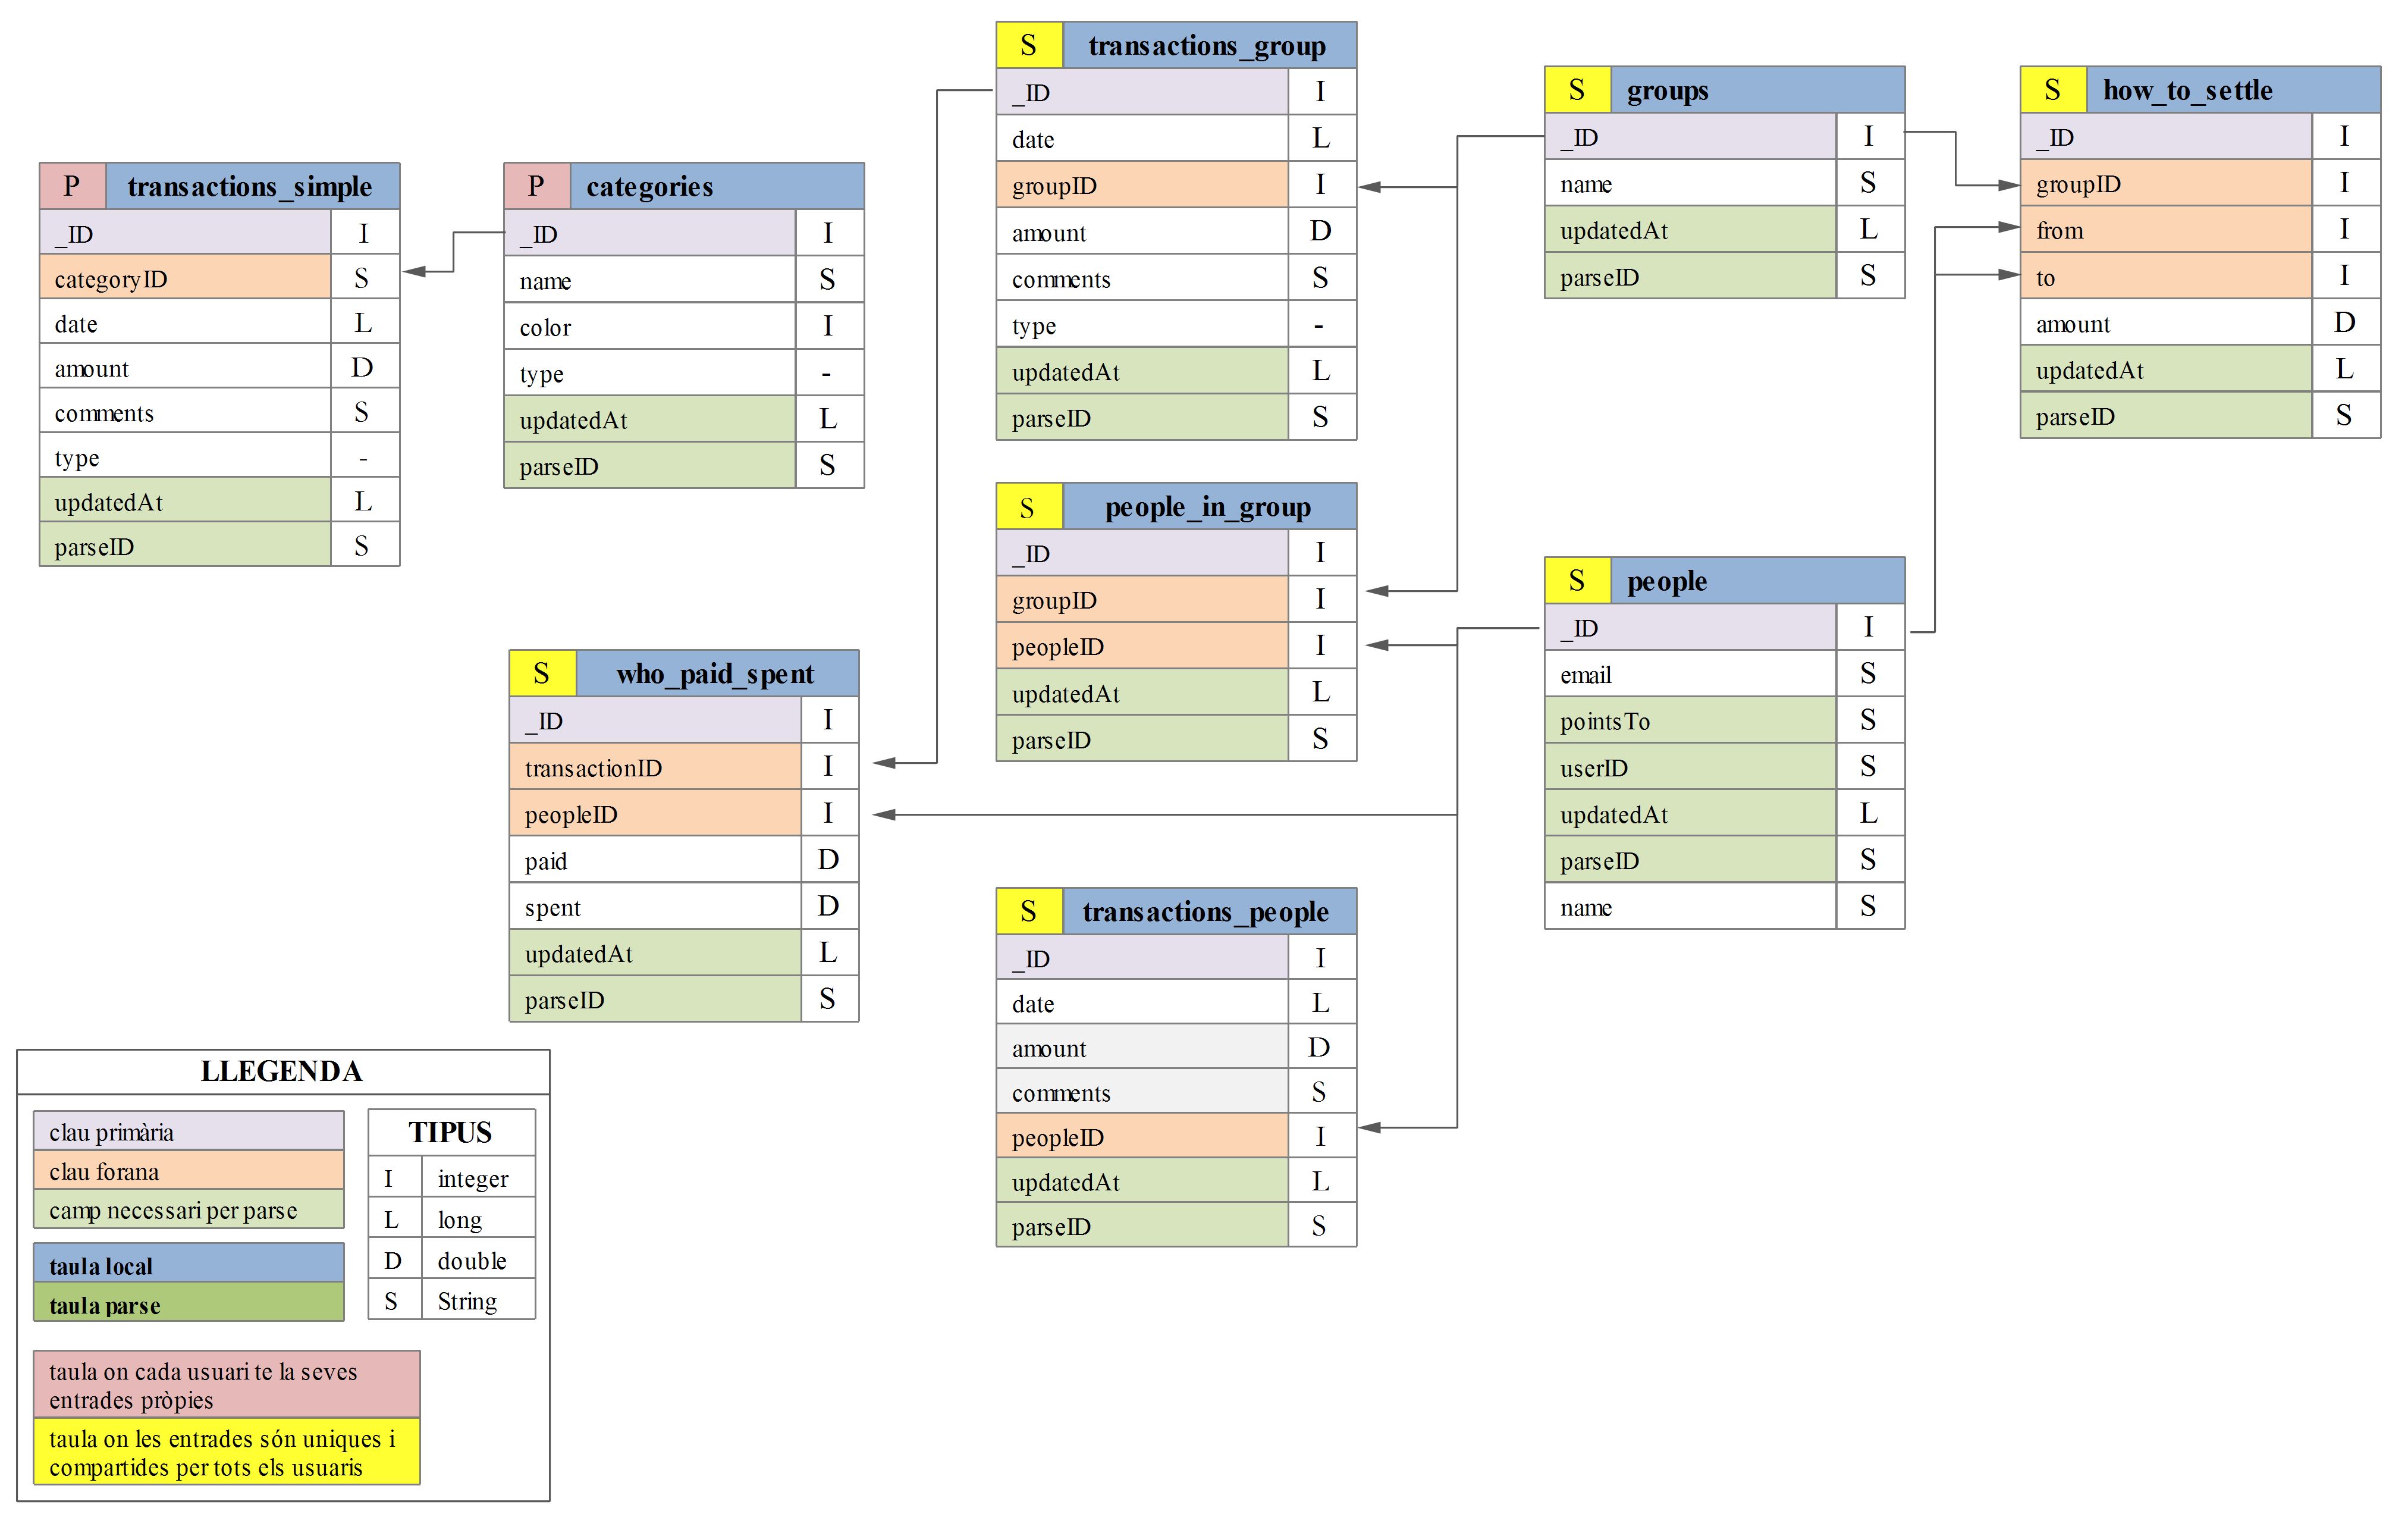
\includegraphics[scale=0.44]{db_sqlite.png}
\caption{Base de dades local amb SQLite}\label{fig:db_sqlite}
\end{figure}

\begin{figure}[ht]
\centering
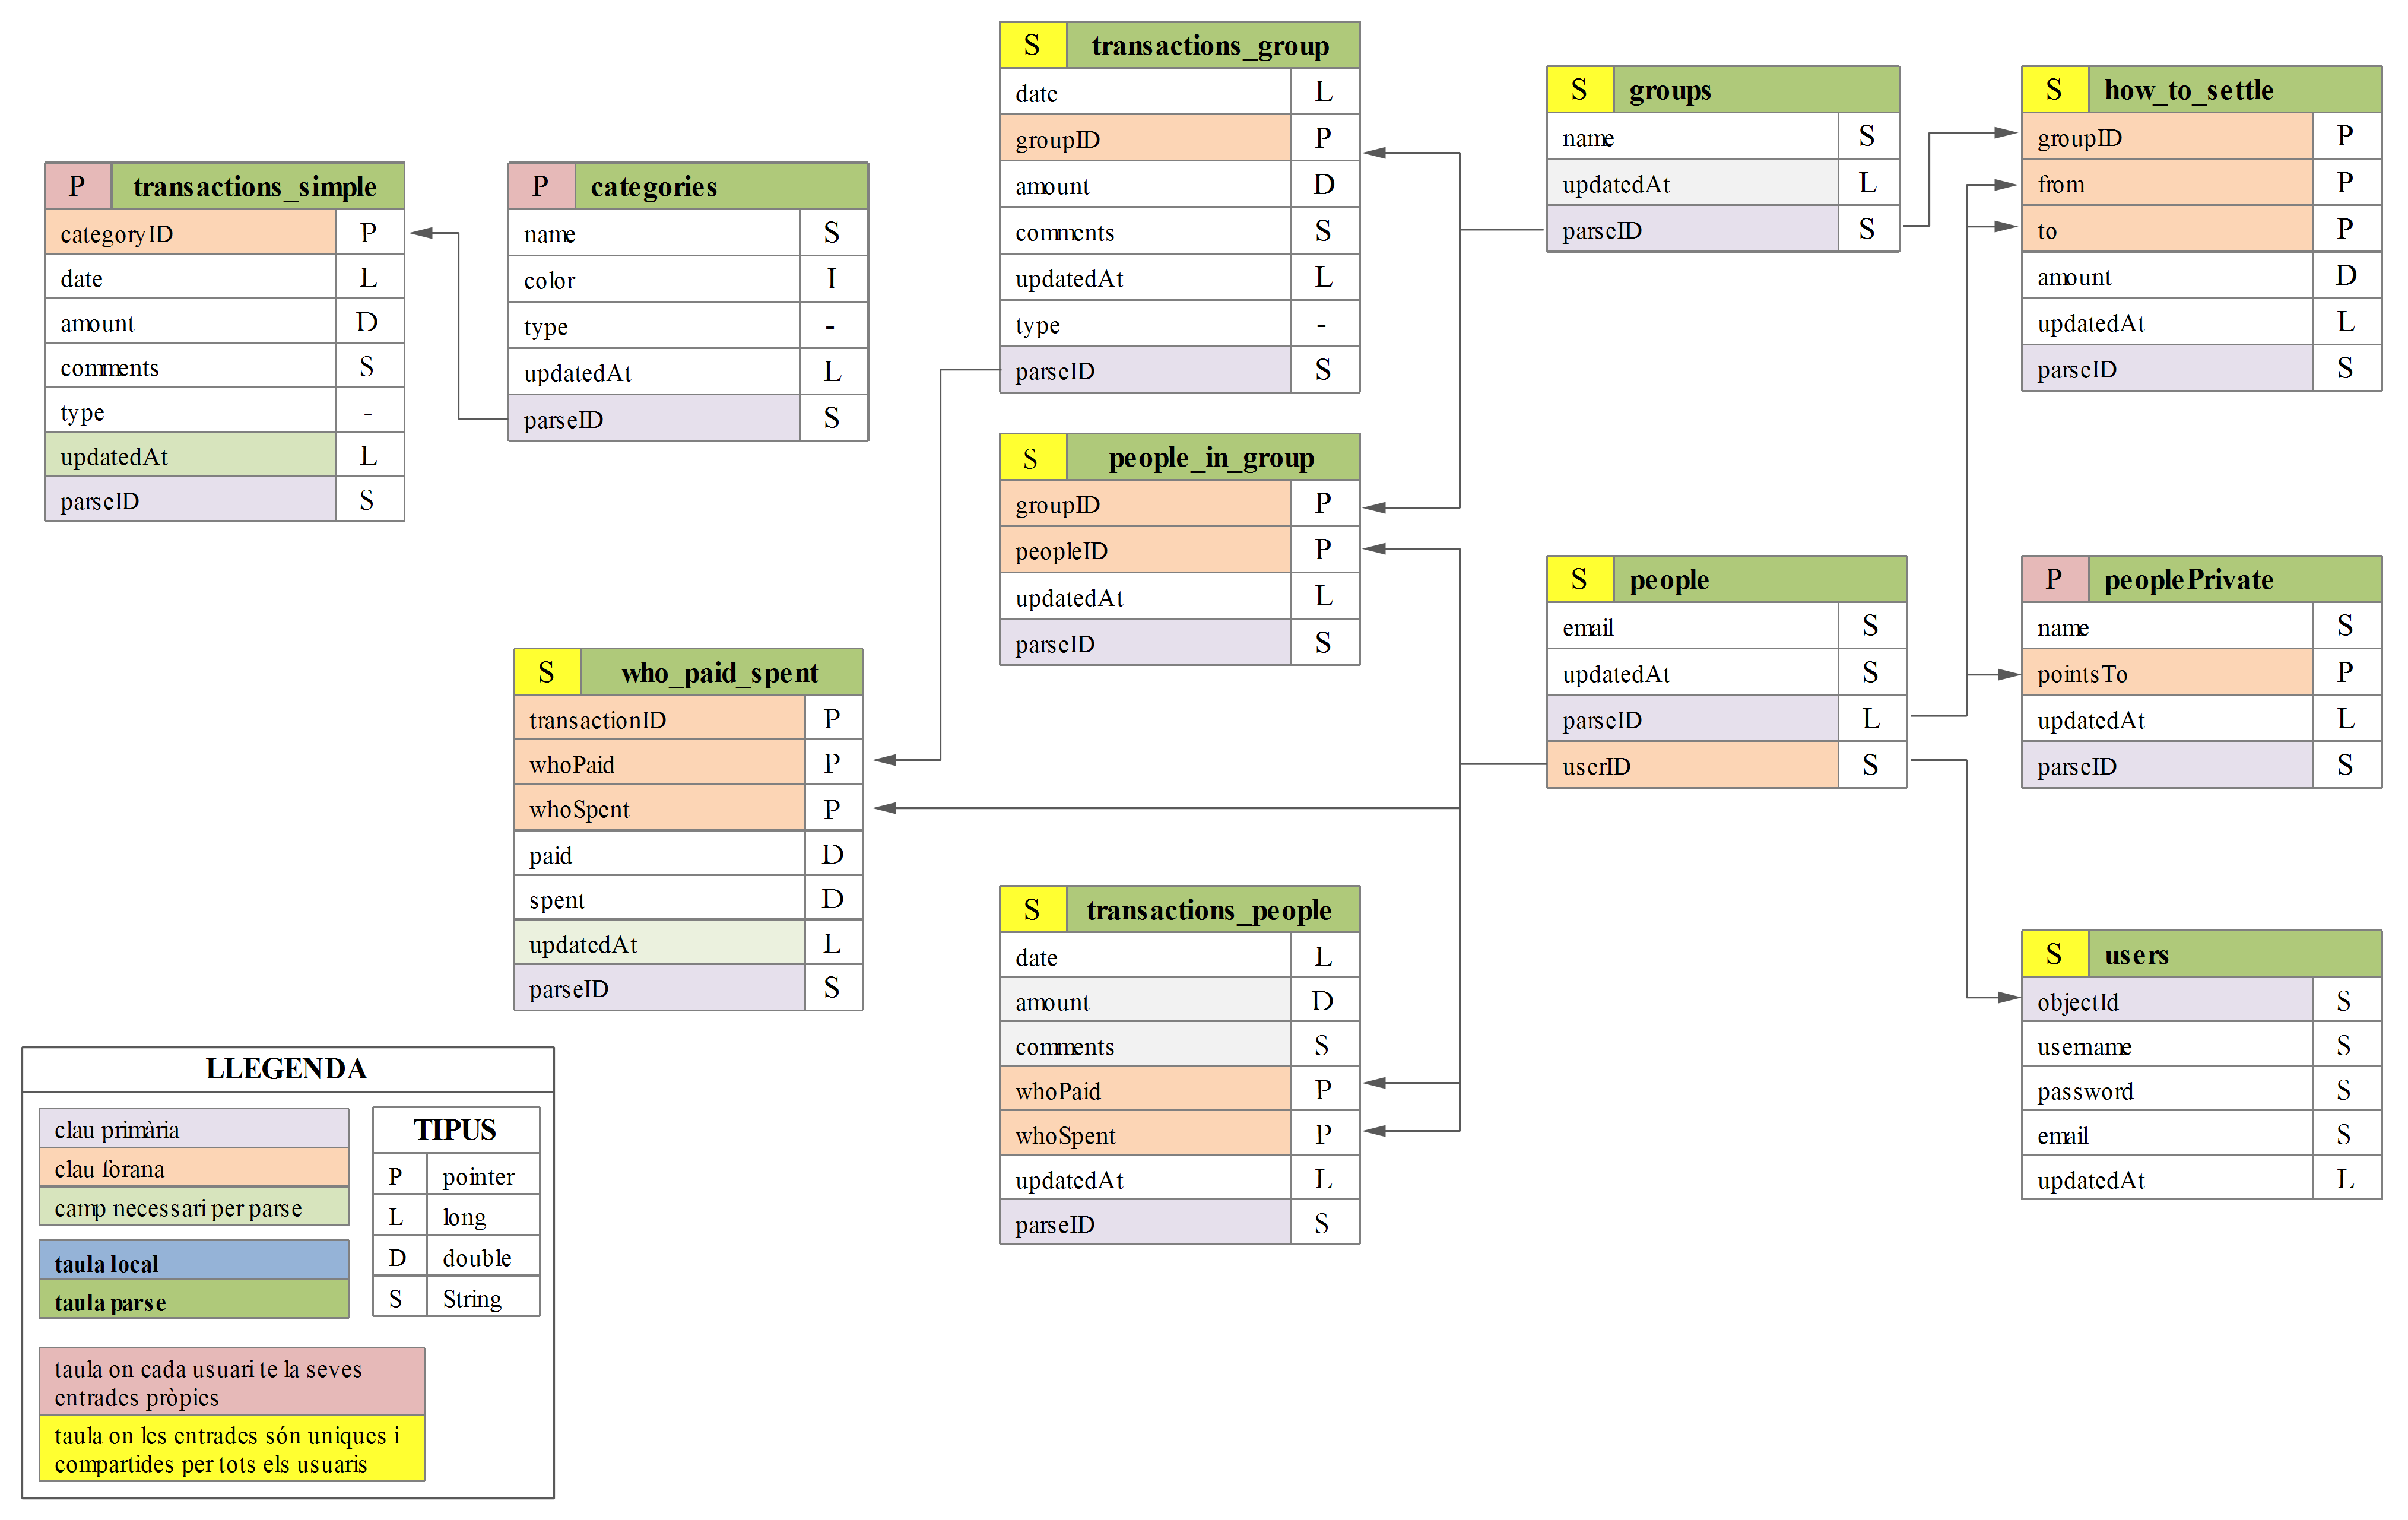
\includegraphics[scale=0.44]{db_parse.png}
\caption{Base de dades al núvol amb Parse.com}\label{fig:db_parse}
\end{figure}

\begin{figure}[ht]
\centering
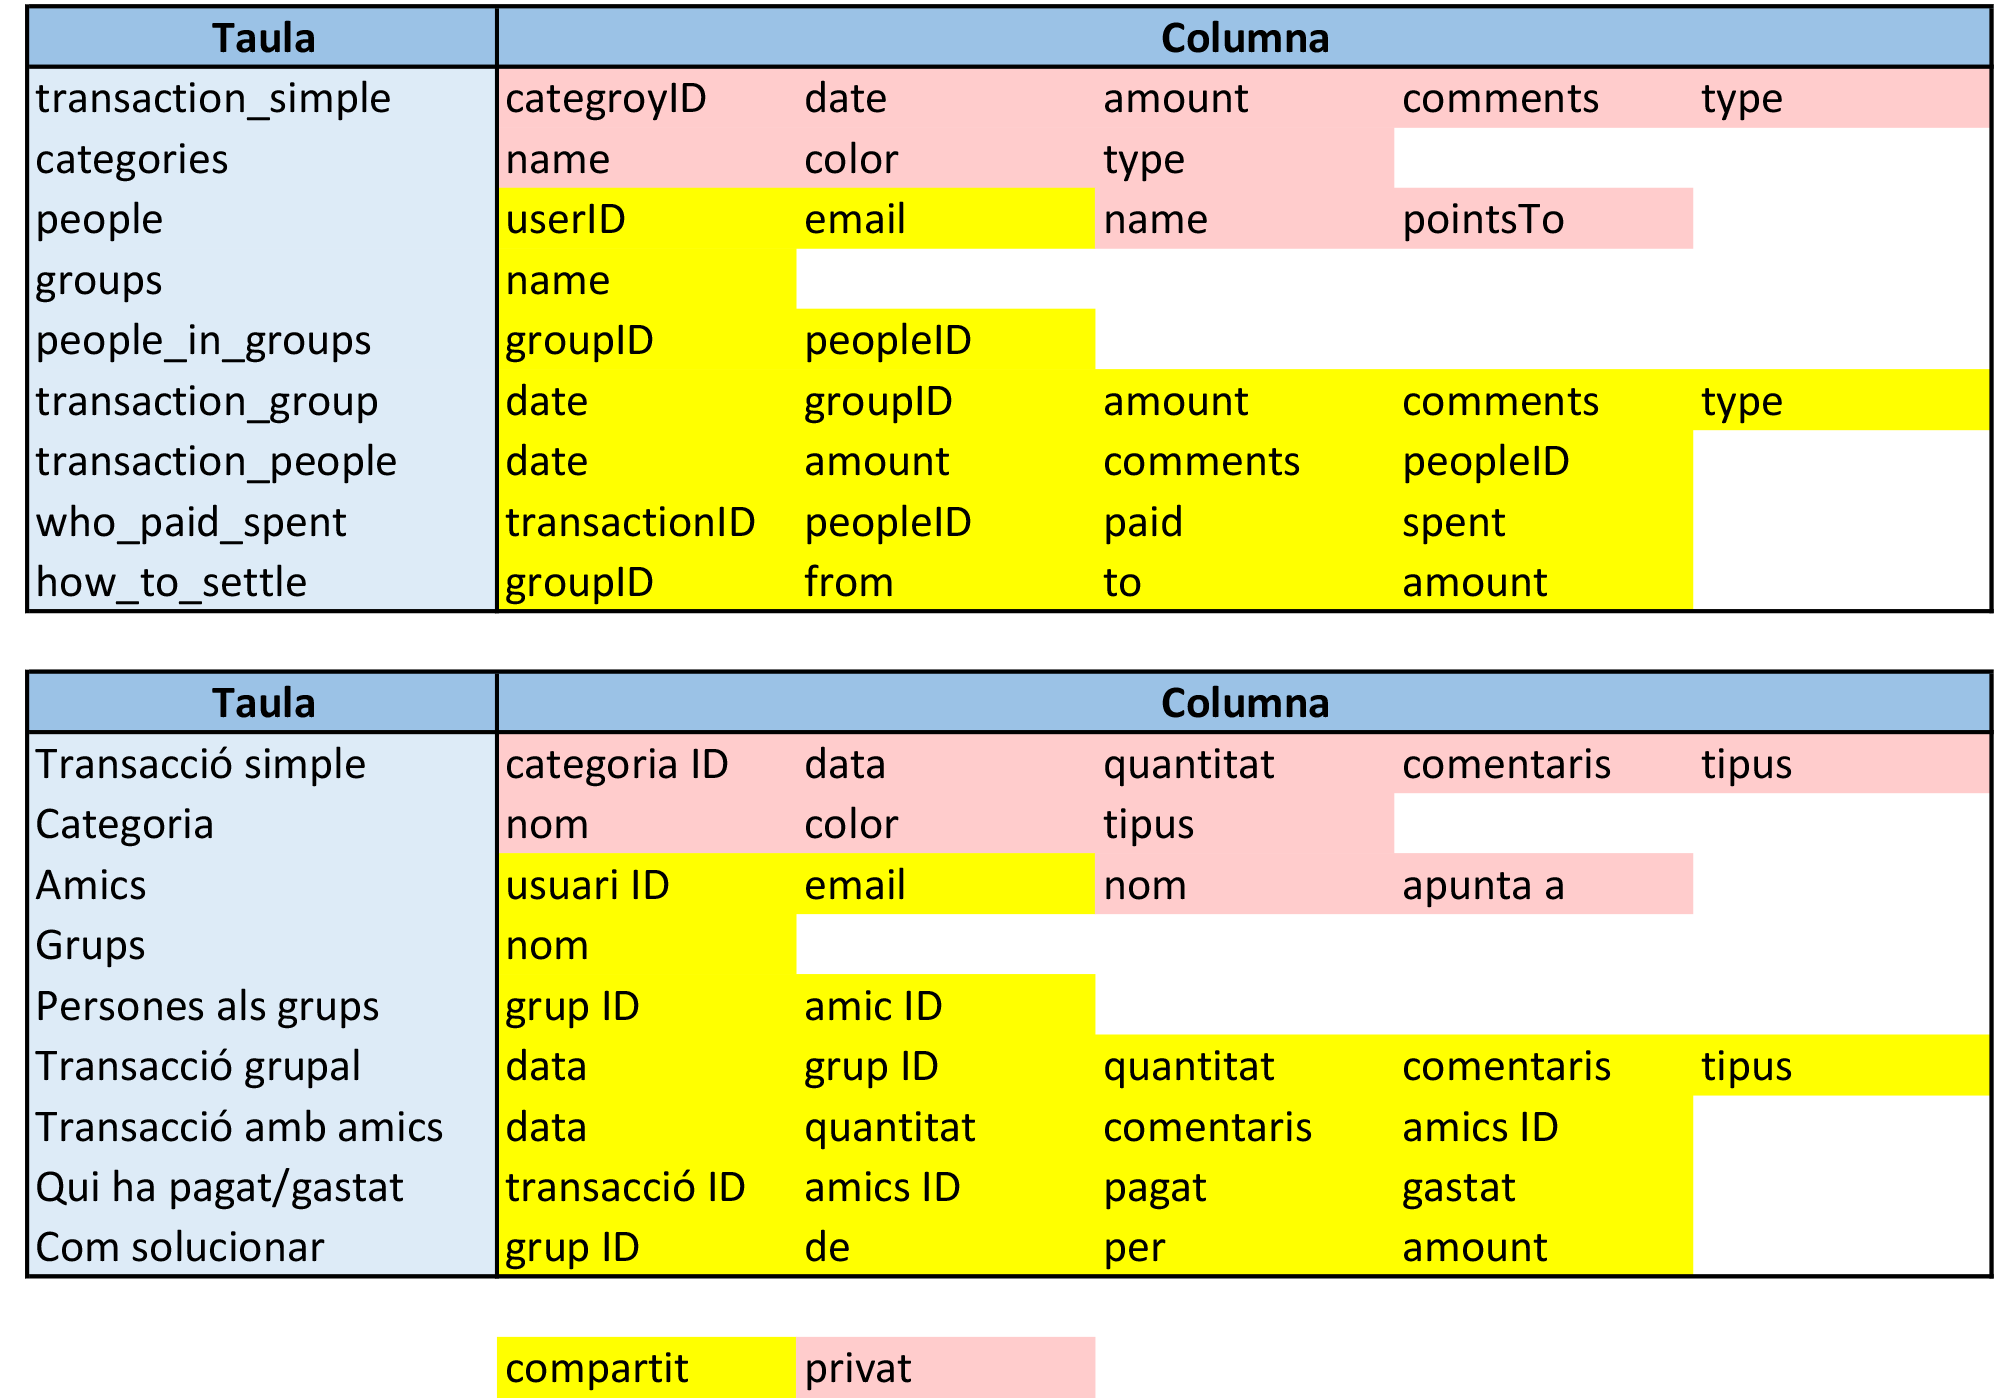
\includegraphics[scale=0.8]{db_private_shared.png}
\caption{Columnes privades i compartides de cada taula}\label{fig:db_private_shared}
\end{figure}


\section{Problema del repartiment de despeses}
Una de les funcions que ha de desenvolupar l'aplicació és fer una proposta sobre com solucionar els deutes existents entre els membres d'un grup. Tot i que en un principi es podria intentar resoldre pensant en les transaccions que ha fet cada membre, a l'hora de solucionar els deutes només cal tenir en compte el balanç de cada persona, tal com exposa David Vávra (creador de l'aplicació Settle Up [veure secció aplicacions \ref{sec:apps}]) a la seva Tesis final de Màster (2012, p. 6-7) \cite{Settle_up}.

Un cop s'analitza el problema es pot veure que s'assembla al típic problema del transport, on s'ha de transportar de les fàbriques als magatzems, amb la diferència qualsevol emparellament té un cost nul i el que es busca és minimitzar el nombre de transaccions. 

Agafem com a exemple les següents persones amb els balanços de la taula \ref{table:balances}.

\begin{table}
\centering
\begin{tabular}{ | l | r |}
\hline
\headB{Persona} & \headB{Balanç} \\
\hline
Arnau & 20,33 \\
\hline
Berta & -3,90 \\
\hline
Càrol & -10,01 \\
\hline
David & 8,57 \\
\hline
Elena & -15,07 \\
\hline
\end{tabular}
\caption{Exemple dels balanços en un grup}
\label{table:balances}
\end{table}


\begin{table}
\centering
\begin{tabular}{ | r | l | r | r |}
 \cline{3-4}
\noBorde{c} & \noBorde{c|} & 20,33 & 8,57 \\
 \cline{3-4}
\noBorde{c} & \noBorde{c|} & \headB{Arnau} & \headB{David} \\
 \hline
 3,9 & \headB{Berta} & & 3,9\\
 \hline
 10,01 & \headB{Càrol} & 5,32 & 4,69\\
 \hline
 15,01 & \headB{Elena} & 15,01 & \\
 \hline
\end{tabular}
\caption{Exemple d'una resolució}
\label{table:resolution}
\end{table}


Es pot veure que la Berta, la Càrol i l'Elena vindrien a ser les fàbriques i que l'Arnau i el David els magatzems als quals s'han d'enviar els diners. A la taula \ref{table:resolution} es mostra el problema juntament amb una solució possible.

Cal notar que degut a arrodoniments al calcular quan ha gastat cada persona en cada transacció és possible que la suma de tots els balanços no sigui 0. S'ha optat per beneficiar als creditors, de manera que tots els deutors paguin tot el que els correspon i que els creditors cobrin tot el que han deixat com a mínim, i si s'escau, alguns decimals de més.

David Vávra proposa solucionar el problema minimitzant només el nombre de transaccions total que s'hauran d'efectuar. Per a fer-ho proposa fer servir un mètode heurístic i posteriorment, si el nombre de persones del grup no es molt elevat, buscar la solució òptima. Per a trobar-la calcula totes les possibilitats. Aquesta manera de resoldre no és el més eficient possible. A més, si s'analitza en més profunditat el problema es pot veure que un bon repartiment no només ha de minimitzar el nombre total de transaccions. Entre altres aspectes que es poden tenir en compte, un bon repartiment serà aquell que:

\begin{itemize}
\item Minimitzi el nombre màxim de transaccions totals
\item Minimitzi el nombre màxim de transaccions que ha de fer una sola persona
\item Si es possible emparelli persones que es coneixen entre elles
\end{itemize}

Una manera de resoldre el problema tenint en compte aquests nous objectius és fent ús de la programació lineal. Concretament es té un de problema de \ac{PLEM}.
%TODO glossary

\subsection{Primera modelització del problema amb resolució exacte}
A continuació es modelarà el problema de solucionar els deutes d'un grup. Per a fer-ho només es buscara que minimitzi el nombre màxim de transaccions totals i el de transaccions que ha de fer una sola persona. Si bé, com ja s'ha dit, una bona solució també tindria en compte l'afinitat entre persones, això és més difícil de modelar i de descobrir sense forçar als usuaris a introduir molta informació. Tot i això la modelització serà prou flexible per a que si en un futur es vol afegir aquest objectiu, es pugui. 
\subsubsection{Dades}
\begin{description}
\item NC = nombre de creditors
\item ND = nombre de deutors
\item $D_{i}=$ diners que deu la persona \textbf{i} $\in (1 \ldots ND)$  [€].
\item $C_{j}=$ diners que li deuen a la persona \textbf{j} $\in (1 \ldots NC)$  [€].
\end{description}


\subsubsection{Variables}
\begin{description}
\item $x_{ij}=$ diners que dona la persona \textbf{i} $\in (1 \ldots ND)$ a la persona \textbf{j} $\in (1 \ldots NC)$  [€].
\item $p_{ij}=$ binaria que indica si la persona \textbf{i} $\in (1 \ldots ND)$ paga a la persona \textbf{j} $\in (1 \ldots NC)$.
\item a = màxim de transaccions dels deutors.
\item b = màxim de transaccions dels creditors
\end{description}

\subsubsection{Restriccions}
\begin{tabular}{l l}
$\sum\limits_{\forall j} x_{ij} \geq D_{i} \quad \forall i$ & Cada deutor ha de pagar com a mínim el que li correspon \\

$\sum\limits_{\forall i} x_{ij} \geq C_{j} \quad \forall j$ & Cada creditor ha de rebre com a mínim el que li correspon \\

$x_{ij} \leq M \cdot p_{ij} \quad \forall i \forall j$ & Forçar valor de $p_{ij}$ (M valor suficientment gran, per exemple $M=\sum\limits_{\forall i} D_{i} + \sum\limits_{\forall j} C_{j})$\\

$\sum\limits_{\forall j} p_{ij} \leq a \quad \forall i$ & Forçar valor de $a$ \\

$\sum\limits_{\forall i} p_{ij} \leq b \quad \forall j$ & Forçar valor de $b$ \\
\end{tabular}

\subsubsection{Funció Objectiu}
[min] $z = \sum\limits_{\forall i \forall j} p_{ij} + \lambda \cdot (a+b)$
Es busca minimitzar el nombre total de transaccions, així com el nombre de transaccions màximes que farà una sola persona
\subsubsection{Paràmetres}
$\lambda$ = usat per decidir el pes a la funció objectiu de cada part

\subsection{Modelització millorada amb resolució exacte}
La modelització anterior en alguns casos no trobava una solució factible, degut als arrodoniments a l'hora de calcular els balanços (pas previ a la solució del \ac{PLEM}).
La idea general d'aquesta modelització es calcular els diners que un deutor pagà a un creditor que formen part del deute per una banda i per l'altre els diners extra que ha de pagar (tot i que no li corresponen). Aquests diners extra sortiran a la funció objectiu amb una penalització molt elevada per tal que al resoldre el \ac{PLEM} només siguin més grans de zero en cas de ser necessari. Vist per la banda dels creditors es farà el mateix, es calcularan els diners extra que han de rebre per tal que els deutors paguin el necessari. De fet aquestes dues variables corresponen a les variables de marge associades a la primera i segona restricció respectivament.

\subsubsection{Dades}
\begin{description}
\item $x_{ij}=$ diners que dona la persona \textbf{i} $\in (1 \ldots ND)$ a la persona \textbf{j} $\in (1 \ldots NC)$  [€].
\item $p_{ij}=$ binaria que indica si la persona \textbf{i} $\in (1 \ldots ND)$ paga a la persona \textbf{j} $\in (1 \ldots NC)$.
\item a = màxim de transaccions dels deutors.
\item b = màxim de transaccions dels creditors
\end{description}

\subsubsection{Variables}
\begin{description}
\item $x_{ij}=$ diners que dona la persona \textbf{i} $\in (1 \ldots ND)$ a la persona \textbf{j} $\in (1 \ldots NC)$  [€].
\item $p_{ij}=$ binaria que indica si la persona \textbf{i} $\in (1 \ldots ND)$ paga a la persona \textbf{j} $\in (1 \ldots NC)$.
\item a = màxim de transaccions dels deutors.
\item b = màxim de transaccions dels creditors 
\item $t_{i}=$ diners extres que ha de pagar la persona \textbf{i} $\in (1 \ldots ND)$  [€].
\item $q_{j}=$ diners extres que ha de rebre la persona \textbf{j} $\in (1 \ldots NC)$  [€].
\end{description}

\subsubsection{Restriccions}
\begin{tabular}{l l}
$\sum\limits_{\forall j} x_{ij} + t_{i} = D_{i} \quad \forall i$ & Cada deutor ha de pagar com a mínim el que li correspon \\

$\sum\limits_{\forall i} x_{ij} + q_{j} = C_{j} \quad \forall j$ & Cada creditor ha de rebre com a mínim el que li correspon \\

$x_{ij} \leq M \cdot p_{ij} \quad \forall i \forall j$ & Forçar valor de $p_{ij}$ (M valor suficientment gran, per exemple $M=\sum\limits_{\forall i} D_{i} + \sum\limits_{\forall j} C_{j})$\\

$\sum\limits_{\forall j} p_{ij} \leq a \quad \forall i$ & Forçar valor de $a$ \\

$\sum\limits_{\forall i} p_{ij} \leq b \quad \forall j$ & Forçar valor de $b$ \\
\end{tabular}

\subsubsection{Funció Objectiu}
[min] $z = \sum\limits_{\forall i \forall j} p_{ij} + \lambda_{1} \cdot \sum\limits_{\forall i} t_{i} + \lambda_{2} \cdot \sum\limits_{\forall j} q_{j} + \lambda_{3} \cdot a + \lambda_{4} \cdot b $

Es busca minimitzar el nombre total de transaccions, així com el nombre de transaccions màximes que farà una sola persona
\subsubsection{Paràmetres}
$\lambda$ = usat per decidir el pes a la funció objectiu de cada part

\subsubsection{Post-procés}
Finalment, per calcular que ha de pagar cada persona es repartiran els diners extres que han de rebre els creditors per tal que tots ells rebin com a mínim tot el que es deu. No es repartiran els diners extres que han de pagar els deutors ja que amb què els creditors rebin el que se'ls hi devia ja n'hi ha prou. Aquests diners extres que un creditor ha de rebre es repartiran entre totes les persones que han de donar-li diners, deixant de banda els deutors que no han de pagar res a aquell creditor. 

Per tant el deutor \textbf{i} pagarà al creditor \textbf{j}: $\frac{x_{ij} + q_{j}*p_{ij}}{\sum\limits_{\forall k} p_{ik}}$

\subsection{Estudi del temps computacional de la modelització millorada}
Un cop es té una bona modelització del problema, cal provar-la amb un aparell i dades reals per comprovar que el temps necessari per resoldre el problema no sigui excessiu. Per a fer-ho s'ha utilitzat un \gls{Nexus_5} i la llibreria per a resoldre problemes de programació lineal \gls{lp_solve}.

En un primer moment s'ha fet servir les dades de 17 balanços provinent de grups de despeses reals creats amb l'aplicació Settle Up. S'ha calculat el temps de resolució per a cada cas 5 cops i s'ha fet la mitjana per cada cas. Analitzant les dades en un primer moment (figura \ref{fig:PLEM_1}) sembla que:

\begin{enumerate}
\item El temps d'execució és sempre molt baix
\item El temps depèn de forma logarítmica del nombre de nodes (N) del problema. ($N = 2*NC*ND + NC + ND + 2$)
\end{enumerate}

\begin{figure}[ht]
\centering
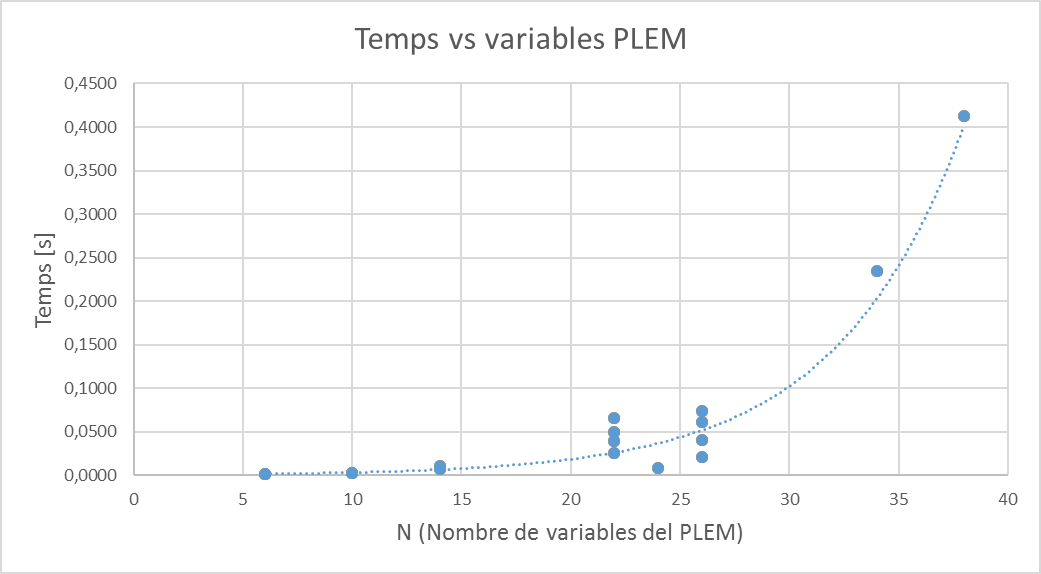
\includegraphics[scale=0.8]{PLEM_temps_2.png}
\caption{Temps per resoldre el PLEM en funció del nombre de nodes (N)}\label{fig:PLEM_1}
\end{figure}

Per a comprovar aquestes hipòtesis s'ha afegit un joc de dades inventat on el nombre de nodes fos més elevat. Amb aquest joc de dades el temps ja no era menor d'un segon (figura \ref{fig:PLEM_2}), com en els altres casos, sinó que estava prop dels 3 minuts. 

\begin{figure}[ht]
\centering
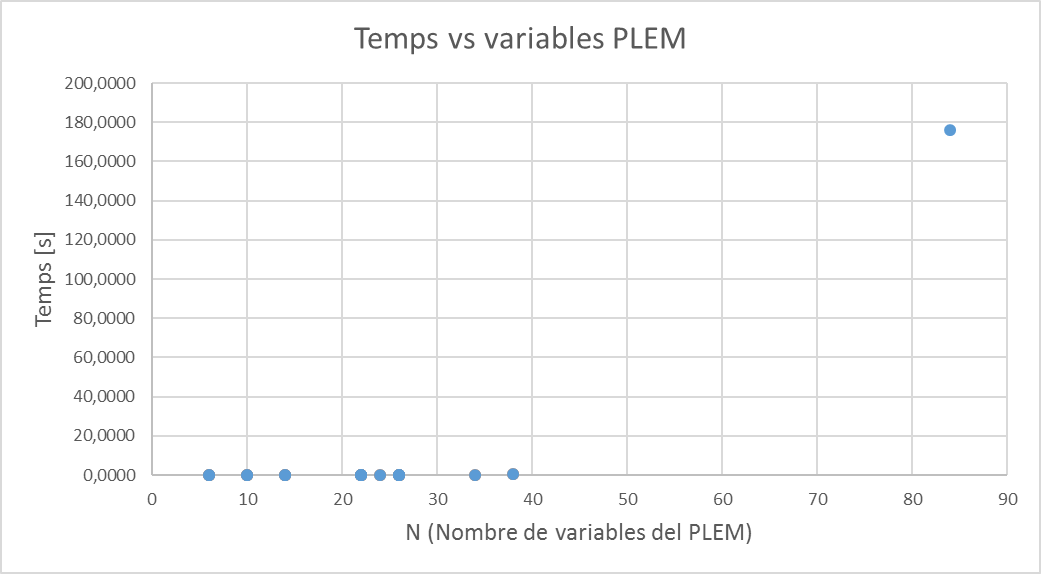
\includegraphics[scale=0.8]{PLEM_temps_1.png}
\caption{Temps per resoldre el PLEM en funció del nombre de nodes (N)}\label{fig:PLEM_2}
\end{figure}

Finalment i després de diverses proves s'ha comprovat que el temps en realitat depèn de forma logarítmica del nombre de deutors i creditors conjuntament, tal com es pot veure a la figura \ref{fig:PLEM_3}. S'han emprat 61 jocs de dades creats de manera que es calculessin la majoria de combinacions possibles de NC i ND amb un temps d'execució relativament baix. Com abans, cada cas s'ha calculat 5 cops i s'ha fet la mitjana dels 5 temps.

%TODO citar les dades

\begin{figure}[ht]
\centering
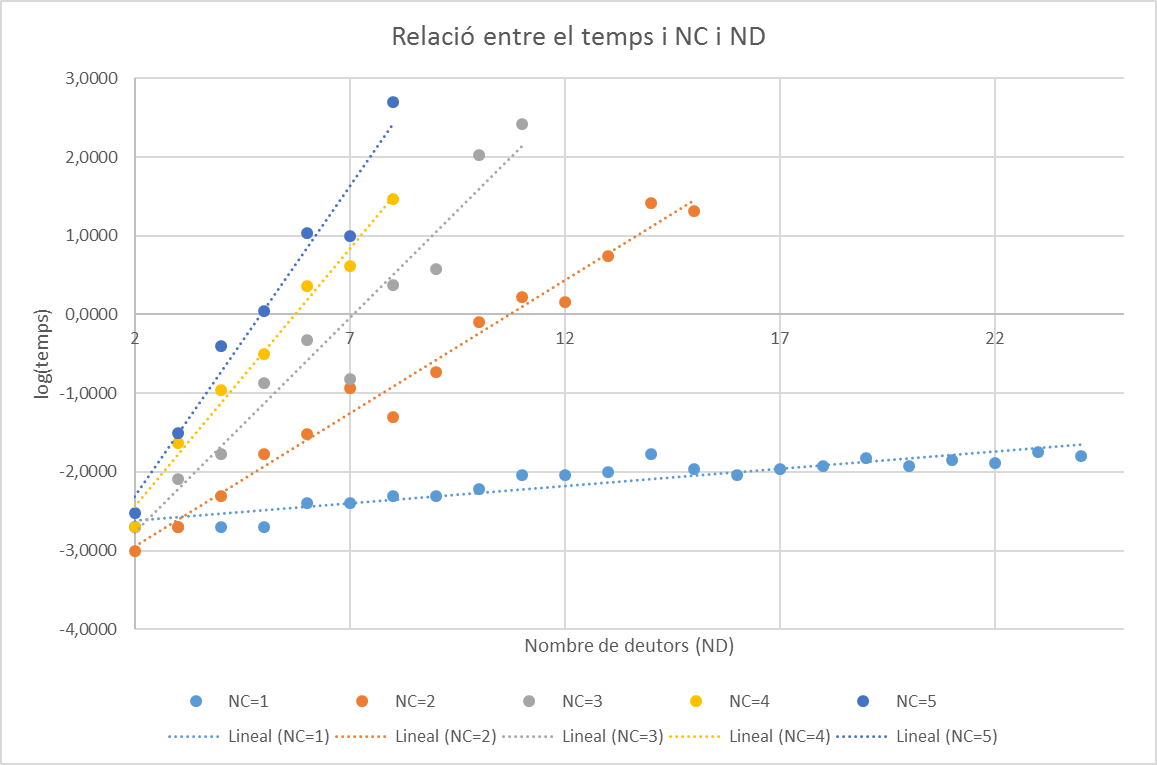
\includegraphics[scale=0.8]{PLEM_temps_3.png}
\caption{Temps per resoldre el PLEM en funció del nombre de creditors (NC) i dels deutors (ND)}\label{fig:PLEM_3}
\end{figure}

Aquest temps d'execució elevat és degut al \gls{BB}. Per trobar una solució amb valors reals, el temps és menor d'un segon, però al intentar trobar una solució amb valors enters tot assegurant què és òptima el temps ja es elevat.

\subsection{Algoritme final}
Finalment s'ha decidit calcular la solució òptima, restringint el programa a un temps d'execució de 3 segons, juntament amb una la resolució heurística que proposa David Vávra (2012, p. 6-7) \cite{Settle_up}. Si en aquest temps el programa troba una solució factible, és compararà amb la solució heurística per veure quin té millor valor de la funció objectiu. Si amb la resolució òptima no s'arriba a una solució factible s'utilitzarà l'aconseguida amb l'heurística. 




\chapter{Impacte ambiental}
% Veure altres projectes: https://upcommons.upc.edu/pfc/?locale=es

\section{Impacte de l'estudi d'Experiència d'Usuari}
El projecte consisteix en un estudi sobre una aplicació per a \gls{smartphone}. El temps invertit en el desenvolupament d'aquest estudi es pot classificar en:

\begin{description}
\item[PFC] Inclou l'anàlisi, disseny i prototipatge (exceptuant els prototips programats), redacció de la memòria, entrevistes amb el tutor etc.
\item[Cursos] Són cursos sobre \gls{Android} i Java que s'han efectuat per poder aprendre a crear aplicacions per aquest sistema.
\item[Programació Android] Inclou el temps invertit programant els diversos prototips i parts d'aquests que han estat programats.
\end{description}


\begin{table}
\centering
\begin{tabular}{ | l | r | r |}
\hline
\headB{Part} & \headB{Temps invertit [h]} & \headB{Consum elèctric [kWh]} \\
\hline
PFC & 281 & 28,08\\
\hline
Cursos & 130 & 13,25\\
\hline
Programació & 471 & 48,00\\
\hline
\end{tabular}
\caption{Hores invertides en l'estudi i consum que representa}
\label{table:impact}
\end{table}

A la taula \ref{table:impact} i a la figura \ref{fig:impact} es poden veure les hores invertides en l'estudi. Durant tot l'estudi s'ha fet servir un ordinador amb una potència mitjana de 100W. A més a més, per a la programació i pels cursos s'ha fet servir un \gls{Nexus_5}, amb una potència mitjana de 2W. 


\begin{figure}[ht]
\centering
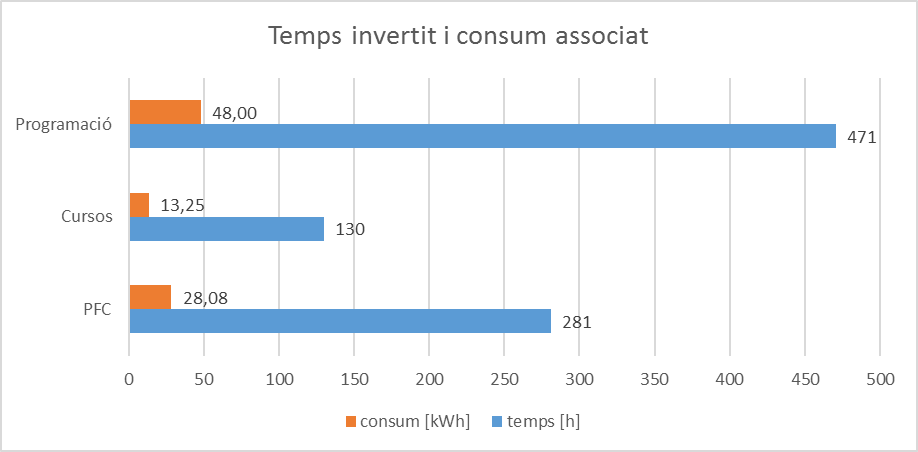
\includegraphics[scale=0.6]{Impact.png}
\caption{Temps invertit i consum associat}\label{fig:impact}
\end{figure}

Apart del consum energètic, també cal considerar el consum de paper. Tot i que s'ha intentat reduir al mínim el seu ús, en algunes parts de l'estudi era necessari, concretament s'ha emprat:

\begin{description}
\item[Plantilles per al disseny:] 22 
\item[Plantilles per a l'avaluació:] 25
\item[Varis:] 5
\end{description}

És a dir, en total s'ha emprat 52 fulls de paper.

\section{Impacte de l'ús de l'aplicació}
Tot i que en aquest projecte només s'ha arribat a crear un prototip, aquest ha estat dissenyat per a que en un futur es pugui posar al mercat una aplicació per a la gestió de despeses domèstiques. Com a tal, s'espera que en un futur modifiqui els hàbits d'alguns usuaris a l'hora de gestionar la seva economia personal, ajudant per una banda a prescindir de l'ús de paper. També s'espera que alguns usuaris canviïn l'ús d'ordinadors per al de \glspl{smartphone} amb el conseqüent estalvi energètic. Això però és més difícil de quantificar ja que depèn de la quantitat d'usuaris que acabin fent servir l'aplicació a més a més del sistema de gestió que utilitzaven prèviament. 


\chapter{Estudi de costos}
En primer lloc a la figura \ref{fig:gantt} es pot veure la planificació de les diverses activitats d'aquest projecte en forma de diagrama de Gantt. L'execució real s'ha adequat a la planificació.

\begin{figure}[ht]
\centering
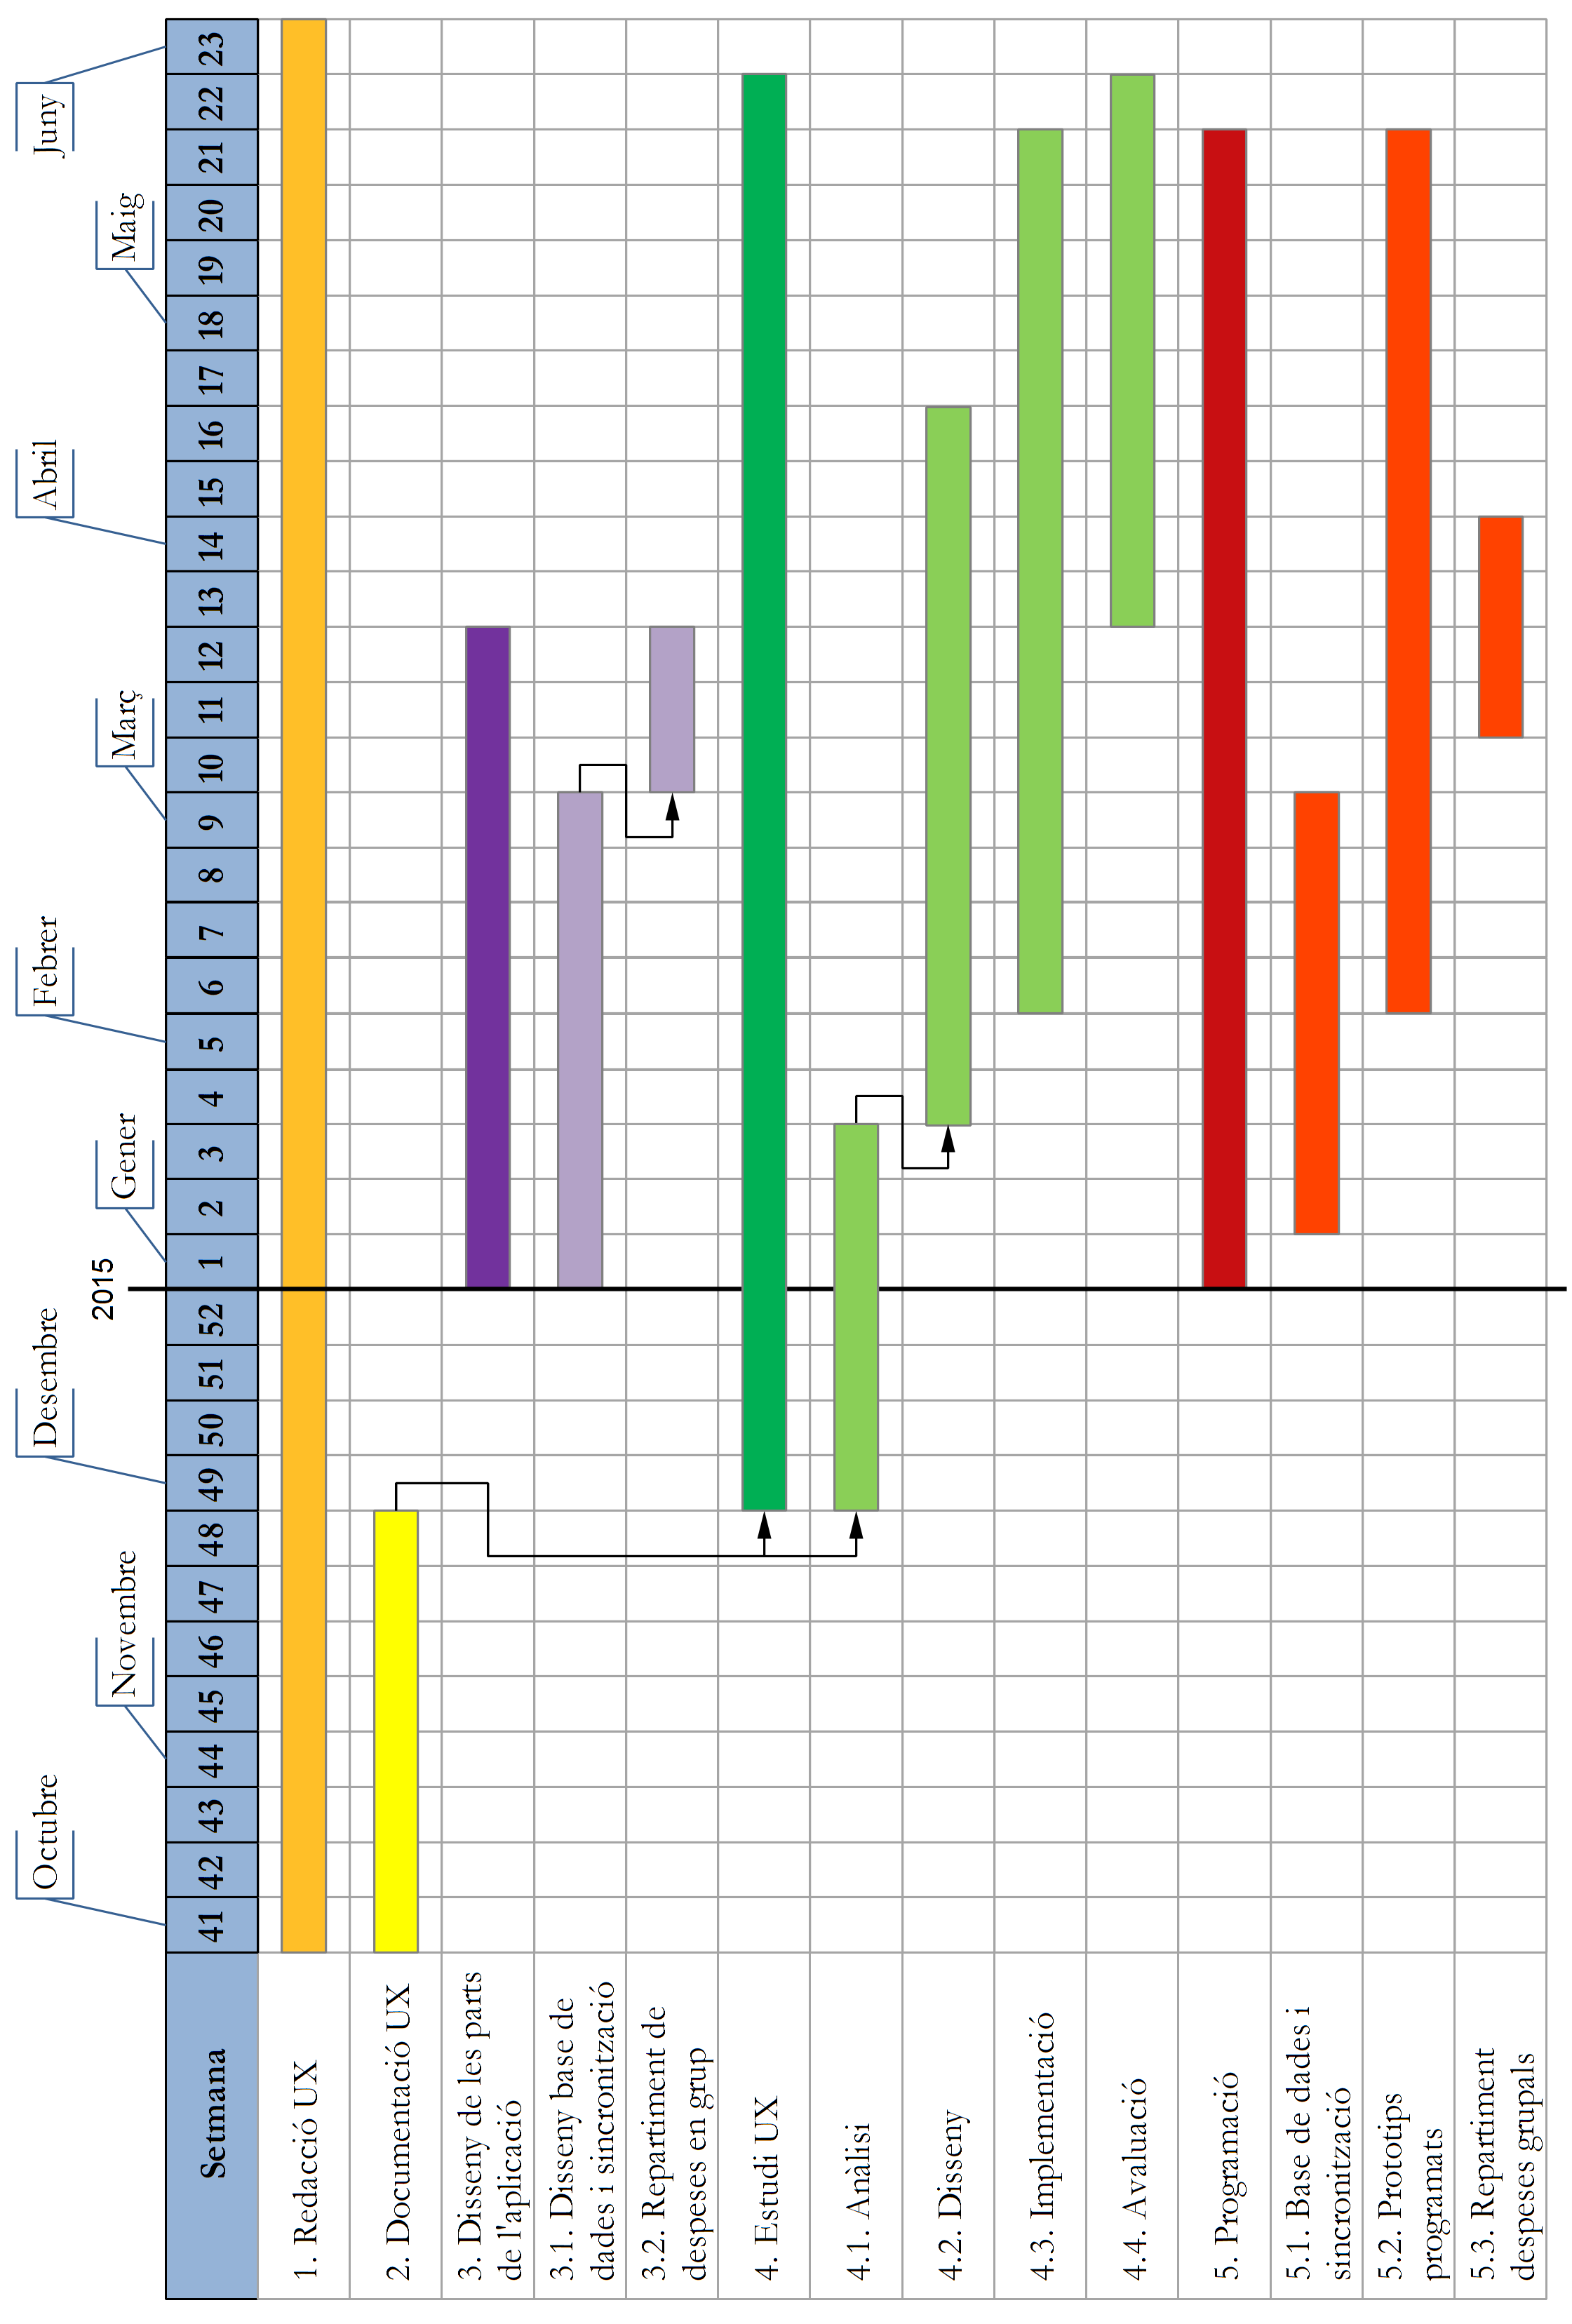
\includegraphics[scale=0.8]{Gantt.png}
\caption{Diagrama de Gantt}\label{fig:gantt}
\end{figure}

De les activitats principals de la figura \ref{fig:gantt} s'extreuen els diversos costos de personal. Per a cada activitat s'han comptabilitzat les hores invertides i, utilitzant el cost per hora, s'ha calculat el cost total de cada activitat, com es pot veure a la taula \ref{table:cost}. 

A més del cost en recursos humans, també s'ha inclòs el cost dels aparells que s'han utilitzat. Per a calcular el cost unitari dels aparells s'ha comptabilitzat el temps que s'han fet servir respecte la seva vida útil. En quan a les llicencies, per a la de \textit{Microsoft Office} s'ha calculat de la mateixa manera que per als aparells. En canvi la llicencia de \textit{Google Play} té un preu únic a pagar per a registrar-s'hi. 

Per al cost de l'energia emprada s'ha fet servir el consum elèctric calculat a l'apartat \ref{impacte}. Fent servir el cost mitjà del kWh a Espanya s'ha calculat el total referent a l'energia emprada.

Finalment el cost total del projecte és de 32.811 \euro { calculat} amb un 21\% d'IVA. El càlcul es pot veure al detall a la taula \ref{table:cost}


\begin{table}[htbp]
  \centering
    \begin{tabular}{| p{4cm} | r | p{3cm} | r | r | r |}
    \hline \headB{Concepte} & \headB{Valor [\euro ]} & \headB{Vida útil [mesos]} & \headB{Unitats} & \headB{Cost unitari} & \headB{Total [\euro ]} \\
    \hline \headA{Personal} & \headA{} & \headA{} & \headA{} & \headA{} & \headA{} \\ \hline
    Redacció PFC &       &       & 66h    & 40 \euro /h   & 2640,00 \euro \\
    Documentació estudis UX &       &       & 57h    & 40 \euro /h   & 2280,00 \euro \\
    Dissenys parts de l'aplicació &       &       & 36h    & 50 \euro /h   & 1800,00 \euro \\
    Estudi UX &       &       & 122h   & 50 \euro /h   & 6100,00 \euro \\
    Programació &       &       & 471h   & 30 \euro /h   & 14130,00 \euro \\
    
    \hline \headA{Aparells} & \headA{} & \headA{} & \headA{} & \headA{} & \headA{} \\ \hline
    Ordinador & 800   & 120   & 8 mesos    & 6,67 \euro /mes & 53,33 \euro \\
    Smartphone Nexus 5 & 350   & 36    & 8 mesos  & 9,72 \euro /mes & 77,78 \euro\\
    
    \hline \headA{Llicencies} & \headA{} & \headA{} & \headA{} & \headA{} & \headA{} \\ \hline
    Google play & 25 \euro   &       &       &       & 25,00 \euro \\
    Microsoft Office 2013 & 119   & 60    &       & 1,98  & 0,00 \euro \\
    
    \hline \headA{Energia} & \headA{} & \headA{} & \headA{} & \headA{} & \headA{} \\ \hline
    Electricitat &       &       & 89,33 kWh & 0,12 \euro /kWh & 10,72 \euro \\
	\hline \headA{Subtotal} & \headA{} & \headA{} & \headA{} & \headA{} & \headA{27116,83 \euro} \\ \hline    
    \hline \headB{Total (IVA 21\%)} & \headB{} & \headB{} & \headB{} & \headB{} & \headB{32811,37 \euro} \\ \hline
    \end{tabular}%
  \caption{Hores invertides, tarifa i cost associat}
\label{table:cost}
\end{table}%



\chapter{Conclusions}

\section{Problema del repartiment de despeses}
Al llarg d'aquest \ac{PFC} s'ha fet un estudi d'\ac{UX} enfocat a una aplicació per a la gestió de despeses personals. En quan als estudis \ac{UX} en si, s'ha deduït:

\begin{itemize}
\item L'anàlisi de com interaccionen els usuaris, sobretot a la primera iteració, és molt útil per entendre que volen els usuaris alhora que permet familiaritzar-se amb el producte/sistema a dissenyar.
\item En quan al disseny i prototipatge és important començar amb una fidelitat i anar incrementant-la a mesura que s'itera. D'aquesta manera s'estalvien molts recursos a les primeres iteracions, i és que no és útil detallar un disseny quan aquest és susceptible de ser canviat. %TODO Flinto al glossari
\item Amb les aplicacions com Flinto (www.flinto.com) es poden animar molt ràpidament dissenys per a crear prototips, però aquests no tindran la flexibilitat dels prototips de paper. En productes/sistemes simples, com l'estudiat, es creu que és suficient amb els prototips creats amb Flinto o semblants, però si el producte/sistema és complex seria millor emprar prototips de paper.
\item Tot i ser un procés iteratiu, si a la primera iteració s'obtenen molt bons resultats s'estalvien molts recursos al llarg de l'estudi. 
\item Pocs usuaris estan disposats a efectuar entrevistes o enquestes llargues. Quants menys productes (dels que ja existeixin) hagin d'avaluar, més usuaris estaran disposats a avaluar-los. 
\item Avaluar 10 aplicacions és pesat per als usuaris, si s'hagués treballat amb 4 o 5 hauria estat millor. Tot i això, al partir l'avaluació sumarial en 2 parts, fent que a la segona només s'avaluessin 3 aplicacions a facilitat obtenir dades de molts usuaris diferents. 
\item A l'avaluació sumarial, uns qüestionaris donen una bona idea de la qualitat obtinguda. Tot i això, si és possible per recursos, és recomanable complementar-ho obtenint mètriques \ac{UX}.
\item Tot i que existeixen moltíssimes aplicacions per gestionar les despeses personals, hi ha poques que garanteixin una bona \ac{UX}. I, evidentment, fer un estudi d'\ac{UX} garanteix que l'aplicació resultat agradi als usuaris. 
\item Un estudi d'\ac{UX} pot ser molt complex i requerir la participació d'un equip molt nombrós. És per això que és important adaptar-lo als recursos disponibles, tant econòmics, com personals o de temps. 
\end{itemize}

En quan a les aplicacions, tant en general com les que serveixen per gestionar despeses, s'ha arribat la conclusió que:

\begin{itemize}
\item Les parts que impliquen més feina al programar sovint són les que els usuaris els hi presten menys atenció, ja que és habitual que les consideren obvies. En aquest cas el repartiment de les despeses grupals ha estat una de les parts més complicades i pocs usuaris li han prestat atenció.
\item Hi ha moltes funcions que no emocionen positivament als usuaris, però que en cas que no funcionin correctament si què tenen un fort impacte negatiu en la seva \ac{UX}. La navegació per l'aplicació n'és un exemple, quan es pot navegar correctament l'usuari ni se n'adona, però en cas que no ho pugui fer es frustrarà.
\item L'apartat visual és molt important pels usuaris, si una aplicació no és maca, és complicat que agradi. Per tant és molt important que qualsevol prototip que vegin els usuaris tingui un bon acabat visual. 
\end{itemize}

I respecte a l'aplicació/prototip creat:

\begin{itemize}
\item S'ha aconseguit crear un prototip bastant semblant a com hauria de ser el producte final.
\item Si bé és cert que no s'ha pogut implementar totes les funcions que havia de tenir l'aplicació, si que comptava amb les funcions més importants, donant una bona idea de com serà l'aplicació si es publica en un futur. %TODO link objectius
\item L'aplicació compleix les funcions esmentades a l'apartat d'objectius encara que li manquin varies funcions que els usuaris volien.
\item El prototip final ha excedit les expectatives si es té en compte que només es creia factible fer proves de concepte.
\item El prototip té alguns errors importants d'\ac{UX} dels quals se'n té constància però que no s'han corregit per manca de temps o coneixements a l'hora de programar. %TODO llista coses a fer app
\end{itemize}

\section{Recomanacions}

\section{Futur de l'estudi/aplicació}
\chapter{Agraïments}

\begin{thebibliography}{9}

%Autor / Titol (Cursiva) / Dades de la publicació
\bibitem{Android_OS}
International Data Corporation. \textit{Smartphone OS Market Share, Q2 2014}. [\url{http://www.idc.com/prodserv/smartphone-os-market-share.jsp}, 20 d'Octubre del 2014].

\bibitem{def_UX}
Rex Hartson. \textit{The UX Book: Process and Guidelines for Ensuring a Quality User Experience}. EEUU: Elseiver, 2012, p. 19.

\bibitem{cant_design_UX}
Smashing Magazine. \textit{User Experience Design}. Alemanya: Smashing Media GmbH, 2012, p. 25-28.

\bibitem{user_centred_design}
Udacity. \textit{Personas and Use Cases Interview with Rich Fulcher}. [\url{https://www.youtube.com/watch?v=uL6xlI17gBU}, 22 de Novembre del 2014]. 

\bibitem{udacity_UX}
Udacity. \textit{UX Design for Mobile Developers}. [\url{https://www.udacity.com/course/ud849}, 22 de Novembre del 2014]

\end{thebibliography}

\end{document}